\def\pascal{0}
\def\preview{1}

%!Tex Root = ../Tutorat1.tex
% ./Design.tex
% ./Deklarationen.tex
% ./Aufgabe1.tex

% https://tex.stackexchange.com/questions/83101/option-clash-for-package-xcolor
% [table]
% https://tex.stackexchange.com/questions/14336/latex-beamer-presentation-package-169-aspect-ratio
% https://tex.stackexchange.com/questions/203045/latex-error-option-clash-for-package-hyperref
% https://stackoverflow.com/questions/3637129/how-can-i-top-align-the-content-of-a-fragile-frame-in-a-latex-beamer-presentat
% https://latex-beamer.com/faq/place-content-frame/
\documentclass[aspectratio=169, hyperref={colorlinks=true, allcolors=PrimaryColor}, c]{beamer}
% t to position content at the top: https://tex.stackexchange.com/questions/9889/positioning-content-at-the-top-of-a-beamer-slide-by-default

% ┌──────────┐
% │ Packages │
% └──────────┘

% \usepackage[margin=1.5cm, headheight=12.5pt]{geometry}
\usepackage[ngerman]{babel}

\usepackage{lipsum}

\usepackage[parfill]{parskip}
% % https://latexref.xyz/bs-par.html
\setlength{\parskip}{0.4cm} % space between paragraphs
% \usepackage{setspace}

% as beamer itself already provides these functionalities, there is no need to load hyperref, color, graphicx, graphics
% \usepackage{graphicx}

% % https://tex.stackexchange.com/questions/48509/insert-list-of-figures-in-the-table-of-contents
% \usepackage[nottoc]{tocbibind}

% % colorbox stuff
\usepackage{tcolorbox}
\usepackage{tikz}
\usetikzlibrary {arrows.meta,positioning}
\usetikzlibrary{graphs}
\tcbuselibrary{skins}
\tcbuselibrary{breakable}
\usetikzlibrary{patterns}
\usetikzlibrary{shadings}
\tcbuselibrary{theorems}
% \tcbuselibrary{listings}
% https://tex.stackexchange.com/questions/550052/command-parboxrestore-has-changed
\tcbuselibrary{minted}
\tcbset{listing engine=minted}
\tcbuselibrary{raster}

% % https://tex.stackexchange.com/questions/547950/highlight-labeled-lines-of-code-with-minted
% % \usepackage{refcount}

% \usepackage{cleveref}

\usepackage[style=authortitle]{biblatex}
\addbibresource{./My Library/My Library.bib}

% \usepackage{pdfpages}
% https://tex.stackexchange.com/questions/94845/problems-with-toprule-and-midrule-in-a-table

\usepackage{booktabs} % for table rules
% % \usepackage{tabulary}
% % https://tex.stackexchange.com/questions/395554/command-rowcolors-from-colortbl-does-not-work-as-expected

\usepackage{nicematrix}
% \usepackage{tabularx}
% \usepackage{array}
% \usepackage{multirow}
% \usepackage{amssymb}

% https://tex.stackexchange.com/questions/157389/how-to-center-column-values-in-a-table
% \newcolumntype{P}[1]{>{\centering\arraybackslash}p{#1}}

% https://stackoverflow.com/questions/2888817/footnotes-for-tables-in-latex
% \usepackage{tablefootnote}

% https://tex.stackexchange.com/questions/8625/force-figure-placement-in-text
% \usepackage{float}

% https://tex.stackexchange.com/questions/219445/line-break-in-texttt
\usepackage{seqsplit}
\newcommand{\seqtt}[1]{{\scriptsize\texttt{\seqsplit{#1}}}}
\newcommand{\smalltt}[1]{{\small\texttt{#1}}}
\newcommand{\tinytt}[1]{{\tiny\texttt{#1}}}
\newcommand{\scripttt}[1]{{\scriptsize\texttt{#1}}}

% https://tex.stackexchange.com/questions/358292/creating-a-subcounter-to-a-counter-i-created
\usepackage{chngcntr}

% https://tex.stackexchange.com/questions/18870/defining-an-new-itemize-like-environment-where-itemfoo-passes-foo-to-a-macro
\usepackage{ifmtarg}


% https://stackoverflow.com/questions/1061112/eliminate-space-before-beginitemize
% https://tex.stackexchange.com/questions/31505/trouble-combining-enumitem-and-beamer
% https://tex.stackexchange.com/questions/325003/given-enumitem-beamer-incompatibility-how-do-i-adjust-the-indent-of-the-enume
% https://tex.stackexchange.com/questions/455692/beamer-presentation-with-itemize-exceed-text-capacity
% \usepackage{enumitem}

% https://tex.stackexchange.com/a/263470
\usepackage{microtype}

% https://tex.stackexchange.com/questions/165178/nameref-hyperref-evaluating-counter-instead-of-section-name
% \usepackage{nameref}

% https://stackoverflow.com/questions/1078370/subfigs-of-a-figure-on-multiple-pages
% \usepackage{subfig}

% https://tex.stackexchange.com/questions/186981/is-there-a-subsubsubsection-command
% https://tex.stackexchange.com/questions/130795/how-can-i-number-sections-below-subsection-in-latex
% \setcounter{secnumdepth}{5}

% % https://stackoverflow.com/questions/2854299/getting-subsection-to-list-in-table-of-contents-in-latex
\setcounter{tocdepth}{4}

% https://tex.stackexchange.com/questions/369421/how-to-have-a-figure-going-over-several-pages
% TODO: set hypcap = true when compiling for the last time
% https://tex.stackexchange.com/questions/132611/change-color-of-figure-caption-text
\usepackage[labelfont={color=SecondaryColor, it}, textfont={it}]{caption}
% hypcap=false

% https://tex.stackexchange.com/questions/7210/label-and-caption-without-float
\DeclareCaptionType{codecaption}[Code][Codeverzeichnis]
% https://tex.stackexchange.com/questions/449677/spaces-in-newenvironment
\newenvironment{code}{\bigskip\captionsetup{type=codecaption}}{\medskip}

% https://texblog.net/latex-archive/uncategorized/prevent-floating-image-figure-table/
% \newcommand\captionof[1]{\def\@captype{#1}\caption}
% \usepackage{capt-of}

% \usepackage{formal-grammar}

% newfloat package
% \SetupFloatingEnvironment{floatgrammar}{name=Grammatik}

% \renewcommand{\downplay}[0]{\rowstyle{\color{gray!90!black}}}
% \newcommand{\removed}[0]{\rowstyle{\color{red}}}

% https://tex.stackexchange.com/questions/26637/how-do-you-get-mathbb1-to-work-characteristic-function-of-a-set
% \usepackage{bbm}
% \usepackage{newtxmath}

% https://tex.stackexchange.com/questions/27843/level-of-boldness-changeable
\usepackage[bold=1]{xfakebold}

% \newcommand{\footnoteurl}[1]{\href{#1}{Link}\footnote{\url{#1}.}}

% https://www.namsu.de/Extra/befehle/Cases.html
\usepackage{mathtools}

\usepackage{breqn}

% https://tex.stackexchange.com/questions/479632/newcommand-combine-optional-star-and-optional-parameter
% \usepackage{xparse}
\tcbuselibrary{xparse}

% https://texfaq.org/FAQ-twooptarg
\usepackage{xargs}

% emojis
% \usepackage{tikzsymbols}

% \usepackage[german]{algorithm2e}

% https://tex.stackexchange.com/questions/237974/hide-section-numbering-but-keep-labeling
% reference titles of sections
% \usepackage[usetoc]{titleref}

% % https://tex.stackexchange.com/questions/531/what-is-the-best-way-to-use-quotation-mark-glyphs
\usepackage{csquotes}

% https://tex.stackexchange.com/questions/326527/colored-blocks-for-numbered-theorems-in-beamer
\usepackage{etoolbox}% new package to be loaded

% https://jansoehlke.com/2010/06/strikethrough-in-latex/
% \usepackage[normalem]{ulem}
% \usepackage{cancel}

%!Tex Root = ../Tutorat3.tex
% ./Packete.tex
% ./Deklarationen.tex
% ./Aufgabe1.tex
% ./Aufgabe2.tex
% ./Aufgabe3.tex
% ./Bonus.tex

% ┌──────────────────────┐
% │ Beamer Configuration │
% └──────────────────────┘

\usetheme{default}
\useoutertheme{infolines}

% ┌─────────────────────┐
% │ Color Configuration │
% └─────────────────────┘

% % https://latexdraw.com/how-to-draw-venn-diagrams-in-latex/
% as beamer itself already provides these functionalities, there is no need to load hyperref, color, graphicx, graphics
% \usepackage{xcolor}
\definecolor{PrimaryColor}{HTML}{5E3072}
\definecolor{PrimaryColorDimmed}{HTML}{a991cc}
\definecolor{SecondaryColor}{HTML}{EC6301}
\definecolor{SecondaryColorDimmed}{HTML}{ffbe99}
\colorlet{BoxColor}{gray!10!white}

\setbeamercolor{normal text}{%
  fg=black,
  bg=white
}
\setbeamercolor{alerted text}{%
  fg=SecondaryColor,
}

% \setbeamercolor{example text}{%
%   fg=PrimaryColor,
% }

\setbeamercolor{structure}{fg=SecondaryColor}

\setbeamercolor{frametitle}{fg=PrimaryColor}
\setbeamercolor{framesubtitle}{fg=SecondaryColor}

\setbeamercolor{title}{fg=PrimaryColor, bg=BoxColor}
\setbeamercolor{subtitle}{fg=SecondaryColor}

% https://github.com/josephwright/beamer/blob/main/base/themes/color/beamercolorthemedefault.sty
% https://github.com/josephwright/beamer/blob/main/base/themes/outer/beamerouterthemeinfolines.sty
\setbeamercolor{author in head/foot}{fg=PrimaryColor, bg=PrimaryColorDimmed}
\setbeamercolor{title in head/foot}{fg=SecondaryColor, bg=SecondaryColorDimmed}
\setbeamercolor{date in head/foot}{fg=PrimaryColor, bg=PrimaryColorDimmed}

\setbeamercolor{palette primary}{fg=PrimaryColor,bg=PrimaryColorDimmed}
\setbeamercolor{palette secondary}{fg=SecondaryColor,bg=SecondaryColorDimmed}
\setbeamercolor{palette tertiary}{fg=PrimaryColor,bg=PrimaryColorDimmed}
\setbeamercolor{palette quaternary}{fg=PrimaryColor,bg=PrimaryColorDimmed}

\setbeamercolor{block title}{fg=white, bg=PrimaryColor}
\setbeamercolor{block body}{fg=black, bg=BoxColor}

\setbeamercolor{block title example}{fg=white, bg=PrimaryColor}
\setbeamercolor{block body example}{fg=black, bg=BoxColor}

\setbeamercolor{block title alerted}{fg=white, bg=SecondaryColor}
\setbeamercolor{block body alerted}{fg=black, bg=BoxColor}

% https://tex.stackexchange.com/questions/326527/colored-blocks-for-numbered-theorems-in-beamer
% https://tex.stackexchange.com/questions/87216/how-to-change-the-color-of-the-text-in-a-theorem-in-beamer/87219#87219
\AtBeginEnvironment{theorem}{% set of commands to be added
    \setbeamercolor{block title}{fg=white,bg=PrimaryColor}% colors to change
    \setbeamercolor{block body}{fg=black,bg=PrimaryColorDimmed}% colors to change
}

\AtBeginEnvironment{proof}{%
    \setbeamercolor{block title}{fg=white,bg=SecondaryColor}
    \setbeamercolor{block body}{fg=black,bg=SecondaryColorDimmed}
}

% https://tex.stackexchange.com/questions/87133/changing-the-color-of-itemize-item-in-beamer
\setbeamercolor{itemize item}{fg=SecondaryColor}
\setbeamercolor{itemize subitem}{fg=SecondaryColor}
\setbeamercolor{itemize subsubitem}{fg=SecondaryColor}

\setbeamercolor{enumerate item}{fg=SecondaryColor}
\setbeamercolor{enumerate subitem}{fg=SecondaryColor}
\setbeamercolor{enumerate subsubitem}{fg=SecondaryColor}

% ┌─────────────────────────┐
% │ Titlepage Configuration │
% └─────────────────────────┘

\newcommand{\titlesecond}{ Aperiodic Scheduling}
\newcommand{\subtitlesecond}{Earliest Deadline Due, Latest Deadline First, Earliest Deadline First}
\newcommand{\type}{
  Exercise class 5\\[-0.25cm]
  \rule{8cm}{0.1mm}
}
\newcommand{\authorsecond}{
  \if\pascal1{Pascal Walter}\else{Jürgen Mattheis}\fi
}
\newcommand{\moreinformation}{
\begin{columns}
\begin{column}{0.5\textwidth}
  \raggedright
  \small
  \emph{In cooperation with:}

  \if\pascal1{Jürgen Mattheis}\else{Pascal Walter}\fi
\end{column}
\begin{column}{0.5\textwidth}
  \raggedleft
  \small
  \emph{Based on the lecture of:}

  Marco Zimmerling
\end{column}
\end{columns}
}
\newcommand{\institutesecond}{University of Freiburg}
\newcommand{\datesecond}{\today}
% \logo{\includegraphics[height=0.5cm]{./figures/logo.png}}

\newcommand{\lehrstuhl}{Chair for Embedded Systems}

\defbeamertemplate*{title page2}{default}[1][]{
  \vbox{}
  \vfill
  \begingroup
    \centering
    \begin{beamercolorbox}[sep=8pt,center,#1]{title}
      \usebeamerfont{title}\titlesecond\par%
      \ifx\subtitlesecond\@empty%
      \else%
        \vskip0.25em%
        {\usebeamerfont{subtitle}\usebeamercolor[fg]{subtitle}\subtitlesecond\par}%
      \fi%
    \end{beamercolorbox}%
    \begin{beamercolorbox}[sep=8pt,center,#1]{institute}
       \type
    \end{beamercolorbox}
    \begin{beamercolorbox}[sep=8pt,center,#1]{author}
      \usebeamerfont{author}\emph{Presenter:}\\ \authorsecond
    \end{beamercolorbox}
    \begin{beamercolorbox}[sep=8pt,center,#1]{institute}
      \moreinformation
    \end{beamercolorbox}\vskip1em
    \begin{beamercolorbox}[sep=8pt,center,#1]{date}
      \usebeamerfont{date}\emph{\datesecond}
    \end{beamercolorbox}
    \begin{beamercolorbox}[sep=8pt,center,#1]{institute}
      \usebeamerfont{institute}\institutesecond, \lehrstuhl
    \end{beamercolorbox}
    {\usebeamercolor[fg]{titlegraphic}\inserttitlegraphic\par}
  \endgroup
  \vfill
}

\makeatletter
\def\titlepagesecond{\usebeamertemplate*{title page2}\@thanks}
\makeatother

\setbeamertemplate{title page2}[default][colsep=-4bp,rounded=true,shadow=true]

% ┌───────────────────────┐
% │ Footline and Headline │
% └───────────────────────┘

% https://github.com/josephwright/beamer/blob/main/base/themes/outer/beamerouterthemeinfolines.sty
\makeatletter
\setbeamertemplate{footline}{%
  \leavevmode%
  \hbox{%
    \begin{beamercolorbox}[wd=.333333\paperwidth,ht=2.25ex,dp=1ex,center]{author in head/foot}%
      \usebeamerfont{author in head/foot}\authorsecond % \expandafter\ifblank\expandafter{\beamer@shortinstitute}{}{~~(\insertshortinstitute)}
    \end{beamercolorbox}%
    \begin{beamercolorbox}[wd=.333333\paperwidth,ht=2.25ex,dp=1ex,center]{title in head/foot}%
      \usebeamerfont{title in head/foot}\titlesecond
    \end{beamercolorbox}%
    \begin{beamercolorbox}[wd=.333333\paperwidth,ht=2.25ex,dp=1ex,leftskip=2ex,rightskip=2ex,sep=0pt]{date in head/foot}%
      \hfill%
      \usebeamerfont{author in head/foot}%
      \institutesecond
      \hfill%
      \usebeamercolor[fg]{page number in head/foot}%
      \usebeamerfont{page number in head/foot}%
      \usebeamertemplate{page number in head/foot}%
    \end{beamercolorbox}
  }%
  \vskip0pt%
}
\makeatother

\setbeamertemplate{headline}{%
\leavevmode%
  \hbox{%
    % https://tex.stackexchange.com/questions/85439/custom-headline-in-latex-beamer
    \begin{beamercolorbox}[wd=\paperwidth,ht=2.5ex,dp=1.125ex]{palette quaternary}%
      \textcolor{PrimaryColor}{\insertsectionnavigationhorizontal{\paperwidth}{\hskip0pt plus1filll}{\hskip0pt plus1filll}}
    \end{beamercolorbox}%
  }
}

% https://tex.stackexchange.com/questions/44983/beamer-removing-headline-and-its-space-on-a-single-frame-for-plan-but-keepin
\newenvironment{withoutheadline}{
  \setbeamertemplate{headline}{%
  \leavevmode%
    \hbox{%
      \begin{beamercolorbox}[wd=\paperwidth,ht=2.5ex,dp=1.125ex]{palette primary}%
      \end{beamercolorbox}%
    }
  }
}{}

\newenvironment{withoutfootline}{
  \setbeamertemplate{footline}{%
  \leavevmode%
    \hbox{%
      \begin{beamercolorbox}[wd=\paperwidth,ht=2.5ex,dp=1.125ex]{palette secondary}%
      \end{beamercolorbox}%
    }
  }
}{}

% ┌──────────────────────┐
% │ Layout Configuration │
% └──────────────────────┘

\setbeamertemplate{blocks}[rounded][shadow=true]

% https://tex.stackexchange.com/questions/578098/number-of-figure-in-beamer
\setbeamertemplate{caption}[numbered]

% \setbeamertemplate{sidebar canvas left}{}
\setbeamersize{sidebar width right=1.5cm}
\setbeamertemplate{sidebar right}{%
  \vspace*{\fill}
  
\includegraphics[width=1.5cm, height=\paperheight]{./figures/background.png}
  \vspace*{\fill}
}

\newcommand{\insertsectionHEAD}{%
	\expandafter\insertsectionHEADaux\insertsectionhead}
	\newcommand{\insertsectionHEADaux}[3]{\LARGE#3
}

\AtBeginSection[] {
  \begingroup
  \setbeamercolor{background canvas}{bg=PrimaryColorDimmed}

  \setbeamertemplate{sidebar right}{%
    \vspace*{\fill}
    
\includegraphics[width=1.5cm, height=\paperheight]{./figures/background.png}
    \vspace*{\fill}
  }

  \begin{frame}
    \centering
    \textcolor{PrimaryColor}{\insertsectionHEAD}
  \end{frame}
  \endgroup
}

% TOC at beginning of each section
% \AtBeginSection[]{
%   \begin{frame}{Gliederung}
%     \tableofcontents[currentsection]
%   \end{frame}
% }

% https://tex.stackexchange.com/questions/87133/changing-the-color-of-itemize-item-in-beamer
\setbeamertemplate{itemize item}[triangle]
\setbeamertemplate{itemize subitem}[triangle]
\setbeamertemplate{itemize subsubitem}[triangle]
% square, circle, triangle, \rightTextArrow

% ┌────────────────────┐
% │ Font Configuration │
% └────────────────────┘

\setbeamerfont{title}{size=\LARGE}
\setbeamerfont{date}{size=\footnotesize}
\setbeamerfont{author}{size=\small}
\setbeamerfont{institute}{size=\small}
\setbeamerfont{subtitle}{size=\large}

\setbeamerfont{frametitle}{size=\LARGE}
\setbeamerfont{framesubtitle}{size=\large}

\setbeamerfont{normal text}{size=\tiny}

% ┌───────────┐
% │ Resources │
% └───────────┘

% - latex beamer templates als Inspiration: https://github.com/benjamin-weiss/hsrmbeamertheme/blob/master/beamerthemehsrm.sty
% - inspiration: https://github.com/martinbjeldbak/ultimate-beamer-theme-list
% - https://github.com/matze/mtheme
% - https://github.com/josephwright/beamer/blob/main/base/themes/color/beamercolorthemedefault.sty
  % - different templates switch
% - https://github.com/josephwright/beamer/blob/main/base/themes/color/beamercolorthemecrane.sty
% - https://github.com/josephwright/beamer/blob/main/base/themes/color/beamercolorthemebeetle.sty
% - https://www.cpt.univ-mrs.fr/~masson/latex/Beamer-appearance-cheat-sheet.pdf
% - (https://git.imp.fu-berlin.de/raup90/swp_2019/-/blob/master/presentation/fu-beamer-template.tex)

%!Tex Root = ../Tutorat3.tex
% ./Packete.tex
% ./Design.tex
% ./Aufgabe1.tex
% ./Aufgabe2.tex
% ./Aufgabe3.tex
% ./Bonus.tex

% ┌──────────┐
% │ Settings │
% └──────────┘

% https://tex.stackexchange.com/questions/325003/given-enumitem-beamer-incompatibility-how-do-i-adjust-the-indent-of-the-enume
% https://tex.stackexchange.com/questions/455692/beamer-presentation-with-itemize-exceed-text-capacity
% \setlist[itemize]{itemsep=2mm, topsep=2mm, parsep=0mm, partopsep=0mm}

% ------------------------------ Minted Settings ------------------------------

% https://tex.stackexchange.com/questions/584071/configure-minted-style-in-latex-for-code-highlighting
% https://pygments.org/docs/tokens/
% https://pygments.org/docs/styledevelopment/#creating-own-styles
% 'custom':  'custom::CustomStyle' in /usr/lib/python3.10/site-packages/pygments/styles/__init__.py
% https://tex.stackexchange.com/questions/18083/how-to-add-custom-c-keywords-to-be-recognized-by-minted#comment930474_42392
\usemintedstyle{custom}

% https://tex.stackexchange.com/questions/345976/global-settings-for-minted
\setminted{fontsize=\tiny,breaklines,highlightcolor=SecondaryColorDimmed,autogobble,escapeinside=||,breakafter={_},breakbefore={(},breakaftersymbolpre={},breakaftersymbolpost={},breakbeforesymbolpre={},breakbeforesymbolpost={},breaksymbolsepleft=2mm,breaksymbolsepright=0mm,breakindent=0mm,breaksymbolindentleft=5mm,breaksymbolindentright=0mm,numbersep=2.5mm}

\newenvironment{linenums}{
  \setminted{linenos}
}{}

% ┌───────┐
% │ Boxes │
% └───────┘

\DeclareTCBInputListing{\codebox}{ s o m }{listing file={#3},
  enhanced,colframe=PrimaryColor,colback=BoxColor,IfBooleanTF={#1}{colframe=SecondaryColor}{colframe=PrimaryColor},fonttitle=\tiny,#2,listing only,halign title=center,drop fuzzy shadow,arc=1mm,bottom=1mm,top=1mm,left=1mm,right=1mm,boxrule=0.5mm,listing engine=minted}
% , sharpish corners

% % https://tex.stackexchange.com/questions/585582/inside-of-a-newtcbinputlisting-how-can-i-change-the-color-of-the-line-number-as
% % https://www.overleaf.com/learn/latex/Using_colours_in_LaTeX
% https://tex.stackexchange.com/questions/132849/how-can-i-change-the-font-size-of-the-number-in-minted-environment
\renewcommand{\theFancyVerbLine}{\ttfamily\textcolor{white}{\tiny{\arabic{FancyVerbLine}}}}
% \renewcommand{\theFancyVerbLine}{\sffamily \textcolor[rgb]{0.5,0.5,1.0}{\huge \oldstylenums{\arabic{FancyVerbLine}}}}

\newtcbinputlisting{\numberedcodebox}[2][]{
  listing file={#2}, enhanced, colframe=PrimaryColor,colback=BoxColor, fonttitle=\small, #1, listing only, halign title=center,drop fuzzy shadow,arc=1mm,boxrule=0.5mm,listing engine=minted,overlay={\begin{tcbclipinterior}\fill[PrimaryColor] (frame.south west) rectangle ([xshift=4mm]frame.north west);\end{tcbclipinterior}}
}

\DeclareTColorBox{codeframe}{ s o m }{
  enhanced, halign title=center, fonttitle=\tiny, interior style={fill=white}, IfBooleanTF={#1}{frame style={color=SecondaryColor}}{frame style={color=PrimaryColor}}, title={#3}, #2,drop fuzzy shadow,arc=1mm,bottom=1mm,top=1mm,left=1mm,right=1mm,boxrule=0.5mm,listing engine=minted,minted style=colorful}

\newtcolorbox{file}[1][]{enhanced, hbox, notitle, interior style={fill=PrimaryColor}, frame empty, halign=center, fontupper=\color{white}\tiny, #1,drop fuzzy shadow,arc=1mm,bottom=1mm,top=1mm,left=1mm,right=1mm,boxrule=0.5mm,listing engine=minted,minted style=colorful}

\newtcblisting{terminal}{
enhanced,colframe=PrimaryColor,colback=BoxColor,hbox,listing only,halign title=center,minted language=text,drop fuzzy shadow,arc=1mm,bottom=1mm,top=1mm,left=1mm,right=1mm,boxrule=0.5mm,listing engine=minted,minted style=colorful,minted options={}}

% % https://tex.stackexchange.com/questions/593218/nested-inline-math-for-new-command-with-argument
\newcommand{\prompt}{\textcolor{SecondaryColor}{\setBold >\;\ignorespaces}}
% % https://tex.stackexchange.com/questions/593218/nested-inline-math-for-new-command-with-argument
\newcommand{\customprompt}{\textnormal\bfseries\textcolor{SecondaryColor}{S}\textcolor{gray!90!black}{he}\textcolor{SecondaryColorDimmed}{ll}\textcolor{SecondaryColor}{>}\;\ignorespaces}

\DeclareTotalTCBox{\inlinebox}{ s v }
{verbatim,colback=SecondaryColorDimmed,colframe=SecondaryColor}
{\IfBooleanTF{#1}%
{\textcolor{SecondaryColor}{\setBold >\enspace\ignorespaces}#2}%
{#2}}

\DeclareTotalTCBox{\key}{ m }
{verbatim,colback=SecondaryColorDimmed,colframe=SecondaryColor}
{$\mathtt{#1}$}

\newtcolorbox{Sidenote}{enhanced,breakable,drop fuzzy shadow,sharpish corners, notitle,arc=0mm,left=3mm,right=3mm,boxrule=1mm, borderline vertical={1mm}{0pt}{PrimaryColor},title=Sidenote,attach boxed title to top text left={yshift=0mm},
interior style={fill=BoxColor},
frame style={color=BoxColor},
% https://tex.stackexchange.com/questions/459870/paragraph-breaks-inside-tcolorbox, maybe also parbox=false
boxed title style={arc=0mm,skin=enhancedfirst jigsaw,frame empty,colback=PrimaryColor,boxrule=0mm,bottom=-0.4mm},
after title={\hspace{0.2cm}
\includegraphics[height=3mm]{./figures/lupe.png}}
}
% before upper=\setlength{\parskip}{1em},
% fonttitle=\bfseries

\numberwithin{equation}{section}

% ┌───────────────┐
% │ Beamer Blocks │
% └───────────────┘

\newcounter{task}
\setcounter{task}{1}

% https://tex.stackexchange.com/questions/309463/beamer-numerating-theorems-and-color-of-block
\setbeamertemplate{theorems}[numbered]

% https://tex.stackexchange.com/questions/152565/define-a-new-block-environment-in-latex-beamer
\renewenvironment<>{task}[1][]{%
  \setbeamercolor{block title}{fg=white,bg=SecondaryColor}%
\begin{block}#2{Task \thesection{.}\thetask:\enspace\ignorespaces #1 \anotebook}}{\end{block}\stepcounter{task}}

% https://tex.stackexchange.com/questions/152565/define-a-new-block-environment-in-latex-beamer
\renewenvironment<>{tasknoinc}[1][]{%
  \setbeamercolor{block title}{fg=white,bg=SecondaryColor}%
\begin{block}#2{Task \thesection{.}\thetask:\enspace\ignorespaces #1 \anotebook}}{\end{block}}

\newenvironment<>{requirements}[1][]{%
  \setbeamercolor{block title}{fg=white,bg=PrimaryColor}%
\begin{block}#2{Requirements \thesection{.}\thetask:\enspace\ignorespaces #1 \anotebook}\itshape}{\end{block}\stepcounter{task}}

\newenvironment<>{requirementsnoinc}[1][]{%
  \setbeamercolor{block title}{fg=white,bg=PrimaryColor}%
\begin{block}#2{Requirements \thesection{.}\thetask:\enspace\ignorespaces #1 \anotebook}\itshape}{\end{block}}

\newenvironment<>{solution}[1][]{%
  \setbeamercolor{block title}{fg=white,bg=PrimaryColor}%
\begin{block}#2{Solution \thesection{.}\thetask:\enspace\ignorespaces #1 \anotebook}\itshape}{\end{block}\stepcounter{task}}

\newenvironment<>{solutionnoinc}[1][]{%
  \setbeamercolor{block title}{fg=white,bg=PrimaryColor}%
\begin{block}#2{Solution \thesection{.}\thetask:\enspace\ignorespaces #1 \anotebook}\itshape}{\end{block}}

% https://stackoverflow.com/questions/34274267/how-can-i-number-theorems-definitions-etc-etc-consecutively-in-latex-without
\newtheorem{customtheorem}{Custom Theorem}[section]
\newtheorem{subcustomtheorem}{Sub Custom Theorem}[customtheorem]
\newtheorem{ocustomtheorem}[customtheorem]{Custom Theorem}

% ┌──────────────┐
% │ New Commands │
% └──────────────┘

% alternative alert
\newcommand\aalert[1]{\textcolor{PrimaryColor}{#1}}

\newcommand{\aitem}{%
\item[\textcolor{PrimaryColor}{$\blacktriangleright$}]\ignorespaces}

% % https://tex.stackexchange.com/questions/8351/what-do-makeatletter-and-makeatother-do
% \makeatletter
%
% % ignorespace: https://runebook.dev/de/docs/latex/_005cignorespaces-_0026-_005cignorespacesafterend
% % enspace: https://math-linux.com/latex-26/faq/latex-faq/article/latex-horizontal-space-qquad-hspace-thinspace-enspace
% \newcommand{\aitem[1]}[]{%
% \@ifmtarg{#1}{\item[\textcolor{SecondaryColor}{\blacktriangleright}]}%
% {\item[\textcolor{SecondaryColor}{\black}] \colorbold{\textbf{#1:}}}\enspace\ignorespaces}
% % \textbullet
%
% \makeatother

\newcommand{\grayitem}{%
\item[\textcolor{gray!90!black}{$\blacktriangleright$}]\ignorespaces}

% https://tex.stackexchange.com/questions/329990/how-do-i-change-the-color-of-itemize-bullet-specific-and-default
% \renewcommand{\labelitemi}{$\textcolor{PrimaryColor}{\bullet}$}
% \renewcommand{\labelitemii}{$\textcolor{PrimaryColor}{\cdot}$}
% \renewcommand{\labelitemiii}{$\textcolor{PrimaryColor}{\diamond}$}
% \renewcommand{\labelitemiv}{$\textcolor{PrimaryColor}{\ast}$}

\newcommand{\notebook}{\hfill
\includegraphics[height=3mm]{./figures/note.png}}
\newcommand{\anotebook}{\hfill
\includegraphics[height=3mm]{./figures/anote.png}}

\newcommand{\magnifier}{\hfill
\includegraphics[height=3mm]{./figures/lupe.png}}

\newcommand\RemoveMargin[2][3em]{%
\makebox[\linewidth][c]{%
  \begin{minipage}{\dimexpr\textwidth+#1\relax}
  \raggedright#2
  \end{minipage}%
  }%
}

% https://tex.stackexchange.com/questions/188379/theorem-numbering-in-beamer
% Nummerierung der Theorem und Berücksichtigung der Sections
\renewcommand\thetheorem{\arabic{section}.\arabic{theorem}}

% ┌──────────────────┐
% │ New Environments │
% └──────────────────┘


\newenvironmentx{transformation}[3][1=0.3, 2=0.2, 3=0.4]{
  \newcommand{\compilesto}{%
    \end{column}\begin{column}{#2\linewidth}\centering$\Rightarrow$\end{column}\begin{column}{#3\linewidth}\centering}
  \newcommand{\arrowx}[1]{%
    \end{column}\begin{column}{#2\linewidth}\centering$\xRightarrow{##1}$\end{column}\begin{column}{#3\linewidth}\centering}
  \newcommand{\arrowxx}[2]{%
    \end{column}\begin{column}{#2\linewidth}\centering$\xRightarrow[##2]{##1}$\end{column}\begin{column}{#3\linewidth}\centering}
  \begin{columns}\begin{column}{#1\linewidth}\centering
  }{%
  \end{column}\end{columns}%
}


\includeonly{
  ./content_Tutorat1/Aufgabe1,
  ./content_Tutorat1/Aufgabe2,
  ./content_Tutorat1/Aufgabe3,
  % ./content_Tutorat1/Aufgabe4,
  ./content_Tutorat1/Bonus,
}

\begin{document}

\begin{withoutheadline}
  \begin{withoutfootline}
    \begin{frame}
      \titlepagesecond
    \end{frame}
  \end{withoutfootline}

  \begin{frame}[shrink=10]{Gliederung}
    \tableofcontents[hideallsubsections]
  \end{frame}
\end{withoutheadline}

\section{Organisation}

\setcounter{section}{-1}

% \if\pascal0{
%   \begin{frame}[allowframebreaks, fragile]{Organisation}
%     \begin{itemize}
%       \item \alert{feedback for me:} \url{https://forms.gle/f3YN8EFrZ1vsfPoC6}
%       \begin{figure}
%         \centering
%         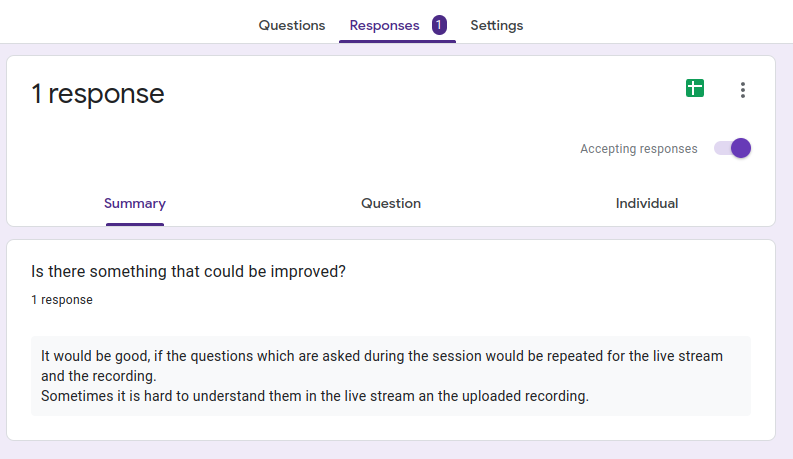
\includegraphics[height=0.3\paperheight]{./figures/feedback.png}
%       \end{figure}
%     \end{itemize}
%   \end{frame}
% }\fi

\section{Overview Aperiodic Task Scheduling}

\begin{frame}{Overview Aperiodic Task Scheduling}
  \centering
  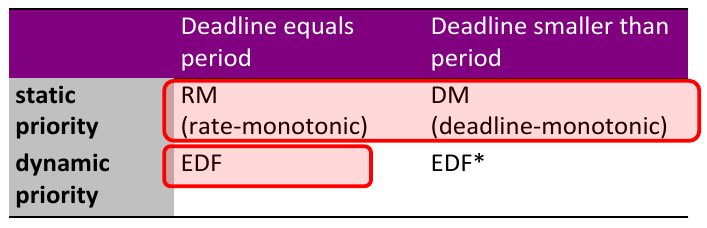
\includegraphics[width=\textwidth]{./figures/overview_real_time_scheduling.png}
\end{frame}

\begin{frame}[shrink=20]{Overview Aperiodic Task Scheduling}{Acceptance Tests\vspace{0.5cm}}
    \begin{NiceTabular}{X[1,l]X[2,l]X[2,l]}[rules/color=PrimaryColor] % {\linewidth}{|C|C|L|L|}
    \CodeBefore
    \chessboardcolors{white}{BoxColor}
    \rowcolor{PrimaryColor}{1}
    \columncolor{PrimaryColor}{1}
    \Body
    & \textcolor{white}{Deadline equals period ($D_i = T_i$)} & \textcolor{white}{Deadline smaller than period ($D_i \le T_i$)} \\
    \textcolor{white}{static priority} & $\displaystyle\sum_{i=1}^n \frac{C_i}{T_i} \leq n\left(2^{1 / n}-1\right)$ \hspace{2cm} (\alert{sufficient} but \alert{not necessary}) & (1) $\displaystyle\sum_{i=1}^n \frac{C_i}{D_i} \leq n\left(2^{1 / n}-1\right)$ \hspace{2cm} (\alert{sufficient} but \alert{not necessary}) \hspace{2cm} (2) smallest $R_i$ that satisfies $\displaystyle R_i=C_i+\sum_{j=1}^{i-1}\left[\frac{R_i}{T_j}\right] C_j$ for all tasks $i$ and $R_i \le D_i$ \hspace{3cm} (\alert{necessary} and \alert{sufficient}) \\
    \textcolor{white}{dynamic priority} & $\displaystyle\sum_{i=1}^n \frac{C_i}{T_i}=U \leq 1$ \hspace{2cm} (\alert{necessary} and \alert{sufficient}) & $\rightarrow$ \cite{buttazzo2011hard} \\
    \bottomrule
  \end{NiceTabular}

\end{frame}

\begin{frame}{Mixed Task Sets}{}
    \begin{itemize}
        \item So far: we differentiated between \alert{periodic} and \alert{aperiodic} tasks.
        \item Now: Consider a \alert{mixed} task set!
        \item We want to be able to find a schedule when there's both \alert{periodic} and \alert{aperiodic} tasks.
    \end{itemize}
\end{frame}

\begin{frame}{Schedulability tests}{Sufficient? Necesarry?}
    \begin{itemize}
        \item We're interested in whether a given problem can be scheduled by algorithms.
        \item Depending on the algorithm we can derive sufficient and necesarry conditions.
        \item[]\alert{Sufficient:} If $A \implies B$ then A is a sufficient condition for B.
        \item[]\alert{Necesarry:} If $B \implies A$ then A is a necesarry condition for B.
        \item A necesarry and sufficient condition means, both statements are logically equivalent.
    \end{itemize}
\end{frame}
\begin{frame}{Schedulability tests}{Utilization}
    Different kind of utilizations also play a big role in our analysis. We introduced the \alert{processor utilization factor} $U = \sum\limits_{i=1}^{n}\cfrac{C_i}{T_i}$ and later on $U_s$ as the server utilization.

    (More about servers later)
\end{frame}
\begin{frame}{RM - Rate Monotonic Scheduling}{Schedulability}
\begin{itemize}
    \item RM is optimal among all fixed-priority assignments in the sense that no other fixed-priority algorithm can schedule a task set that cannot be scheduled by RM.
    \item As in the lecture, we have $\sum\limits_{i=1}^{n}\cfrac{C_i}{T_i} \leq n(2^{1/n}-1)$ as a \alert{sufficient} but not \alert{necesarry} condition.
\end{itemize}
\end{frame}
\begin{frame}{RM(PS) - Rate Monotonic Polling Server}
    \begin{itemize}
        \item One way to handle both periodic and aperiodic tasks is to use a so called server.
        \item This PS (Polling Server) acts as a periodic task (meaning it is instantiated at regular intervals $T_s$) whose job it is to, once it has the highest priority, serve any pending aperiodic requests within the limits of a server capacity $C_s$.
        \item Since we introduce yet another periodic task, the schedulability analysis simply is the same as normal $RM$ with one additional task. Again, we have the \alert{sufficient} but not \alert{necesarry} condition: $\cfrac{C_s}{T_s} + \sum\limits_{i=1}^{n}\cfrac{C_i}{T_i} \leq (n+1)(2^{1/(n+1)}-1)$
    \end{itemize}
\end{frame}

% \begin{frame}{EDF - Total Bandwidth Server}
%
% \end{frame}


% \begin{frame}{Overview Aperiodic Task Scheduling}
%   \begin{itemize}
%     \item \alert{Lateness:} $L_i = f_i - d_i$
%     \item \alert{Maximum lateness:} $\displaystyle L_{\max }=\max_i\left(f_i-d_i\right)$
%     \begin{itemize}
%       \item this a a metric to compare schedules
%     \end{itemize}
%   \end{itemize}
% \end{frame}
% %
% \begin{frame}{TT Cyclic Executive Scheduling}{Recap: Definitions}
%     \begin{itemize}
%         \item $\Gamma:$ set of all periodic tasks
%         \item $\tau_i:$ one particular periodic task (the i-th)
%         \item $\tau_{i,j}:$ the $j$th instance of task $i$
%         \item $r_{i,j}:$ release time of $j$th instance of task $i$
%         \item $d_{i,j}:$ absolute deadline of the $j$th instance of task $i$
%         \item $\Phi_i:$ phase of task $i$
%         \item $D_i:$ relative deadline of task $i$
%     \end{itemize}
% \end{frame}
%
% \begin{frame}{TT Cyclic Executive Scheduling}{Recap: Three assumptions}
% \begin{enumerate}
%     \item The instances of a periodic task are regularly activated at a constant rate. The interval between two consecutive activations is called period. The release times satisfy $r_{i,j} = \Phi_i + (j-1)T_i$
%     \item All instances have the same worst case execution time $C_i$ (also written as $WCET(i)$)
%     \item All instances of a periodic task have the same relative deadline $D_i$. Therefore the absolute deadlines satisfy $d_{i,j} = \Phi_i + (j-1)T_i + D_i$
% \end{enumerate}
% \end{frame}

%!Tex Root = ../Tutorat1.tex
% ./Packete.tex
% ./Design.tex
% ./Deklarationen.tex
% ./Aufgabe2.tex
% ./Aufgabe3.tex
% ./Bonus.tex

\section{Task 1 - Memory map}

\begin{frame}{Task 1 - Memory Map}{Task 1.1}
  \begin{solution}
    \begin{columns}
      \begin{column}{0.2\textwidth}
        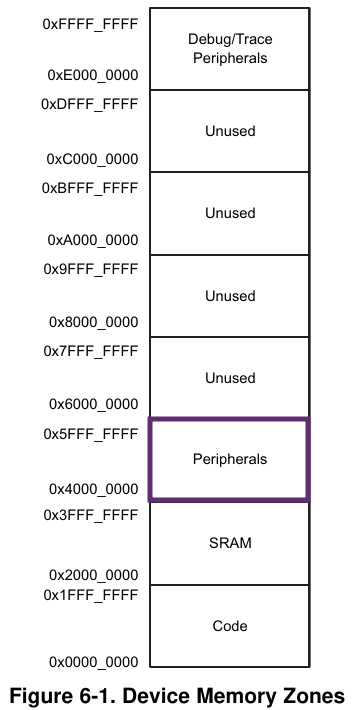
\includegraphics[height=0.5\paperheight]{./figures/peripherals.png}
      \end{column}
      \begin{column}{0.8\textwidth}
        \begin{itemize}
          \item $0x5FFF\_FFFF - 0x4000\_0000 + 1 = 0x2000\_0000$
          \item $0x2000\_0000 = 2 \cdot 16^7 = 2 \cdot {(2^4)}^7 = 2 \cdot 2^{4\cdot 7} = 2^{1+28} = 2^{29}$
        \end{itemize}
      \end{column}
    \end{columns}
  \end{solution}
\end{frame}

\begin{frame}{Task 1 - Memory Map}{Task 1.1}
  \begin{solution}
    \begin{columns}
      \begin{column}{0.4\textwidth}
        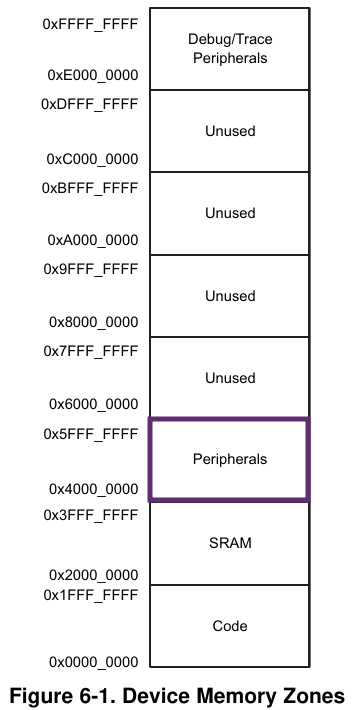
\includegraphics[height=0.5\paperheight]{./figures/peripherals.png}
        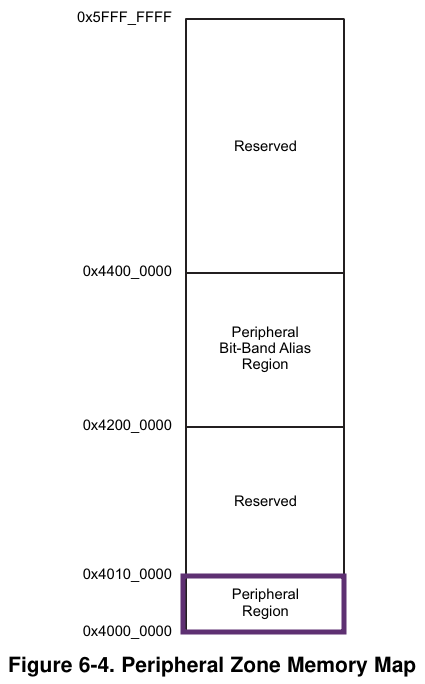
\includegraphics[height=0.5\paperheight]{./figures/peripherals_region.png}
      \end{column}
      \begin{column}{0.6\textwidth}
        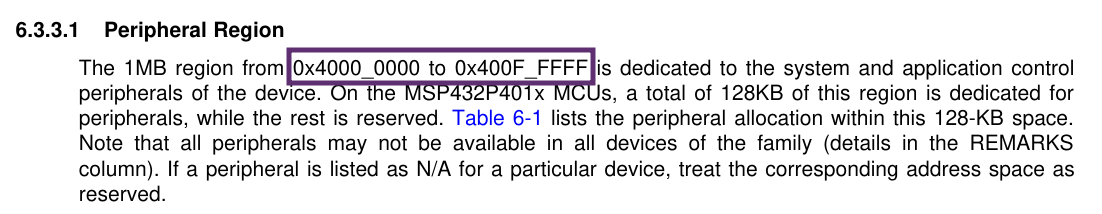
\includegraphics[width=0.5\paperwidth]{./figures/system_and_application_control_peripherals.png}
        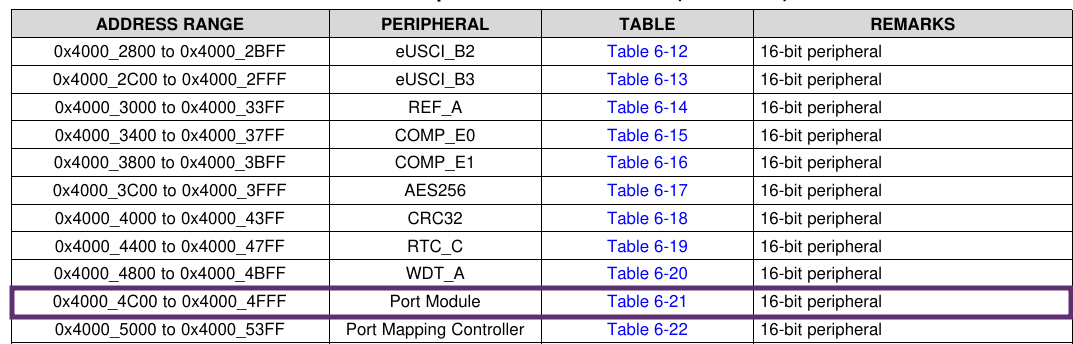
\includegraphics[width=0.5\paperwidth]{./figures/port_module.png}
      \end{column}
    \end{columns}
    \begin{itemize}
      \item $0x4000\_4FFF - 0x4000\_4C00 + 1 = 0x0400$
      \item $0x0400 = 4 \cdot 16^2 = 2^2 \cdot {(2^4)}^2 = 2^2 \cdot 2^{(4\cdot 2)} = 2^{2+8} = 2^{10}$
    \end{itemize}
  \end{solution}
\end{frame}

\if\preview0{
\begin{frame}[allowframebreaks]{Task 1 - Memory Map}{Task 1.1}
  \begin{solution}
    \begin{columns}
      \begin{column}{0.4\paperwidth}
        \centering
        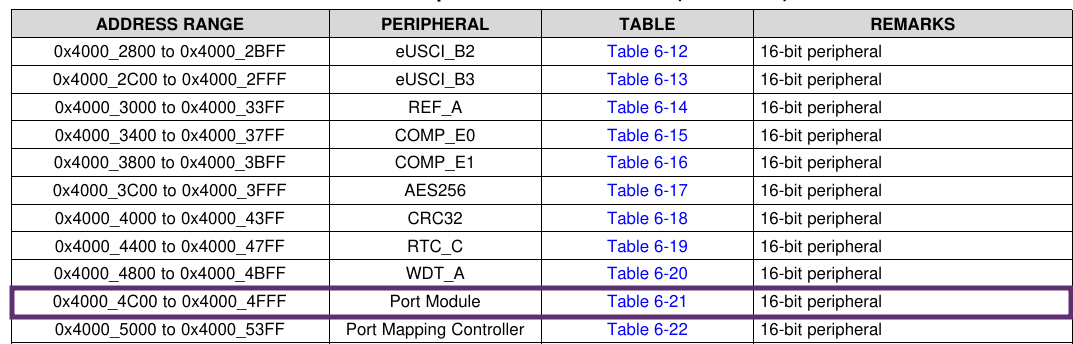
\includegraphics[width=0.3\paperwidth]{./figures/port_module.png}
        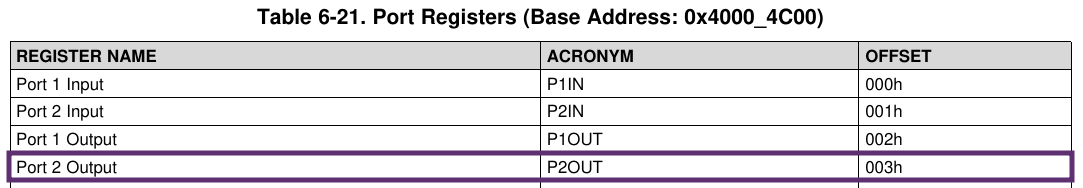
\includegraphics[width=0.3\paperwidth]{./figures/port2.png}
        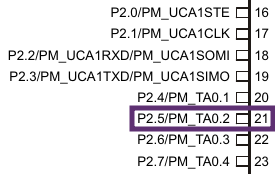
\includegraphics[height=0.2\paperheight]{./figures/2_5.png}
      \end{column}
      \begin{column}{0.6\paperwidth}
        \begin{itemize}
          \item $0x4000\_4C00 + 0x0003 = 0x4000\_4C03$
          \item 6th least significant bit $\Rightarrow$ $0b0010\_0000$
        \end{itemize}
      \end{column}
    \end{columns}
  \end{solution}
  \begin{Sidenote}
    \begin{itemize}
      \item 003h is an alternative way to write 0x0003
    \end{itemize}
  \end{Sidenote}
\end{frame}

\begin{frame}[allowframebreaks]{Task 1 - Memory Map}{Task 1.1\vspace{0.25cm}}
  \begin{solutionnoinc}
    \begin{columns}
      \begin{column}{0.3\paperwidth}
        \centering
        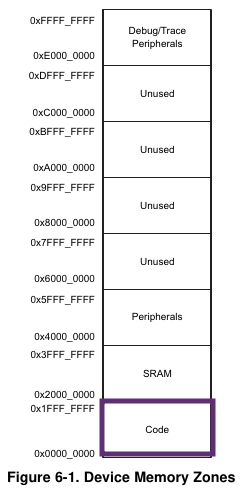
\includegraphics[height=0.4\paperheight]{./figures/code.png}
        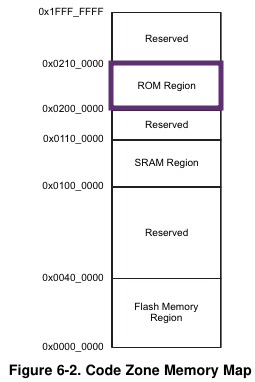
\includegraphics[height=0.4\paperheight]{./figures/rom.png}

      \end{column}
      \begin{column}{0.7\paperwidth}
        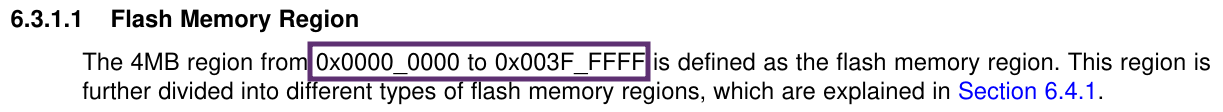
\includegraphics[height=0.095\paperheight]{./figures/rom2.png}
        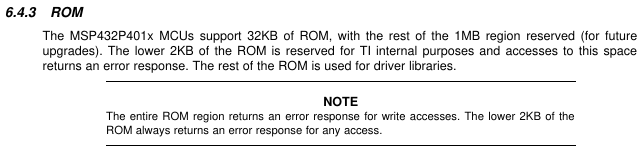
\includegraphics[height=0.25\paperheight]{./figures/rom3.png}
      \end{column}
    \end{columns}
    \begin{itemize}
      \item $0x020F\_FFFF - 0x0200\_0000 + 1 = 0x0010\_0000$.
      \item $16^5 = {(2^4)}^5 = 2^{4\cdot 5} = 2^{20} \text{addresses}$
    \end{itemize}
  \end{solutionnoinc}
  \begin{solution}
    \begin{itemize}
      \item each address location corresponds to \alert{one byte} $\Rightarrow$ \alert{addressable memory space} is $2^{20} Byte$ or $1 MiB$.
      \item number of 4-byte words is a \alert{quarter} of that, which is $\frac{2^{20} Byte}{2^2} = 2^{18} words = 2^8 Kiwords= 256 Kiwords$
    \end{itemize}
  \end{solution}
  \begin{Sidenote}
    \begin{itemize}
      \item developer can not write to these addresses, only the manufacturer can (ROM = \alert{R}ead-\alert{o}nly \alert{m}emory)
      \item the MSP432P401x MCUs supports 32KB of ROM, and the rest of the 1MByte ROM region is reserved for \alert{future upgrades}
    \end{itemize}
  \end{Sidenote}
\end{frame}
}\fi

\begin{frame}{Task 1 - Memory Map}{Task 1.2\vspace{0.25cm}}
  \begin{figure}
    \centering
    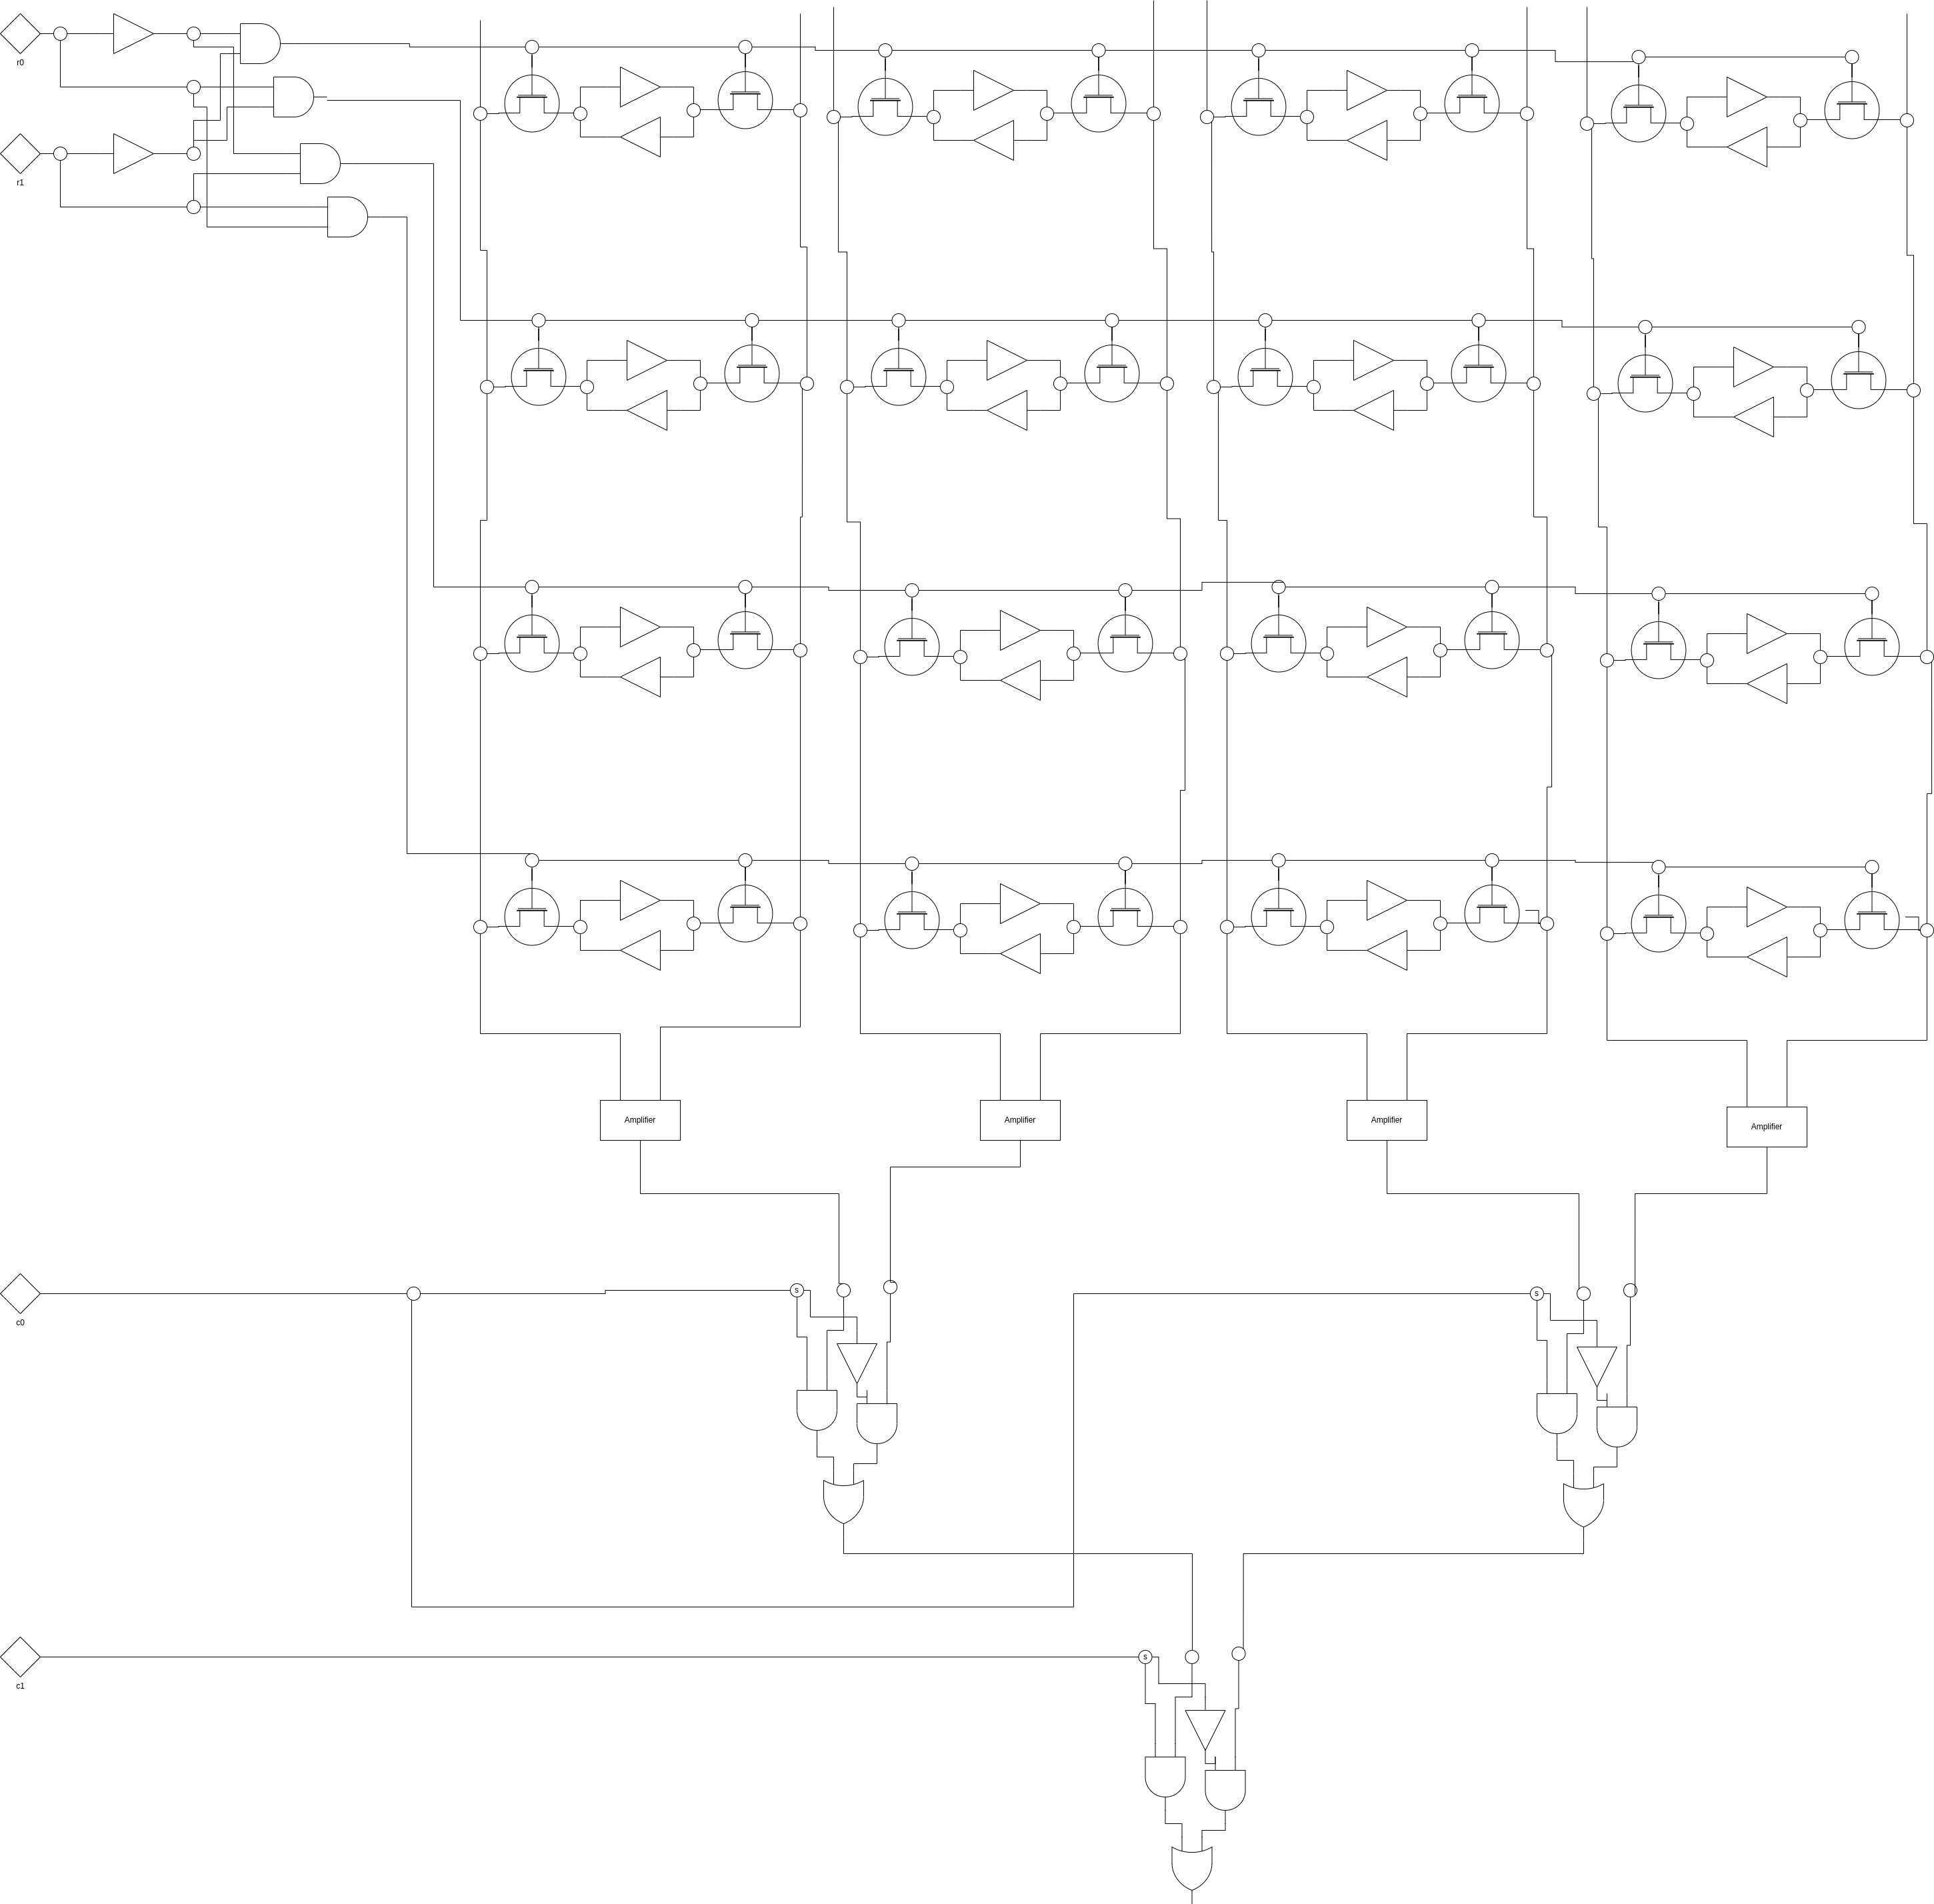
\includegraphics[height=0.6\paperheight]{./figures/sram.png}
    \caption{SRAM-cell array}
  \end{figure}
\end{frame}

\begin{frame}{Task 1 - Memory Map}{Task 1.2\vspace{0.25cm}}
  \begin{itemize}
    \item $u$ \alert{row} select bits and $w$ \alert{column} select bits
    \item \alert{we need:}
    \begin{itemize}
      \item $2^{(u+w)}$ memory cells
      \item one $u$-bit decoder
      \item one $2^w$-to-$1$ multiplexer
      \item $2^w$ sense amplifiers
    \end{itemize}
  \end{itemize}
\end{frame}

\begin{frame}{Task 1 - Memory Map}{Task 1.2\vspace{0.25cm}}
  \begin{figure}
    \centering
    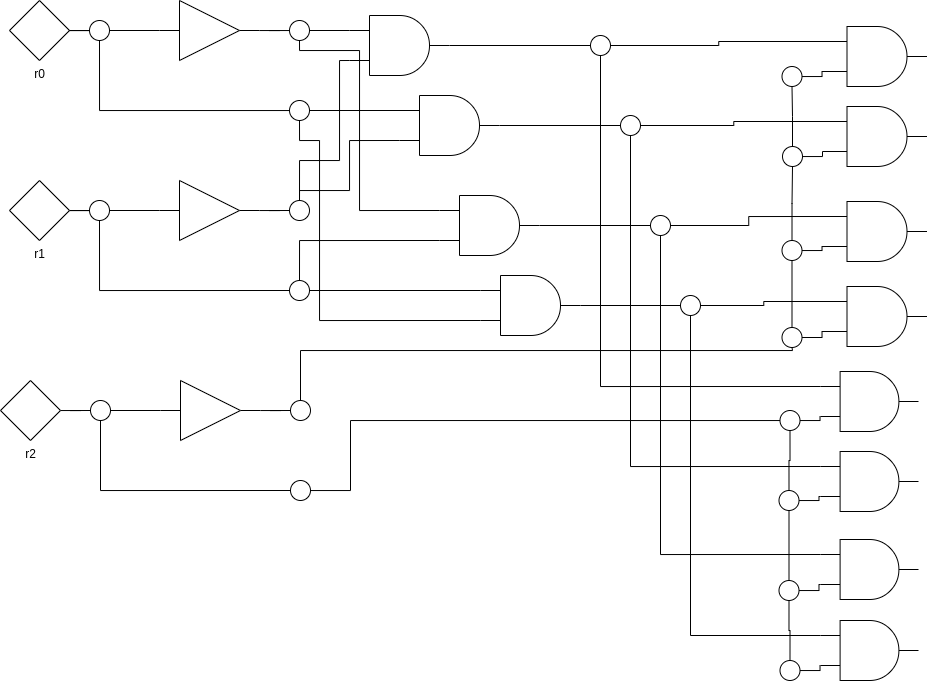
\includegraphics[height=0.6\paperheight]{./figures/3BitDecoder.png}
    \caption{3-Bit Decoder}
  \end{figure}
  % \begin{figure}
  %   \centering
  %   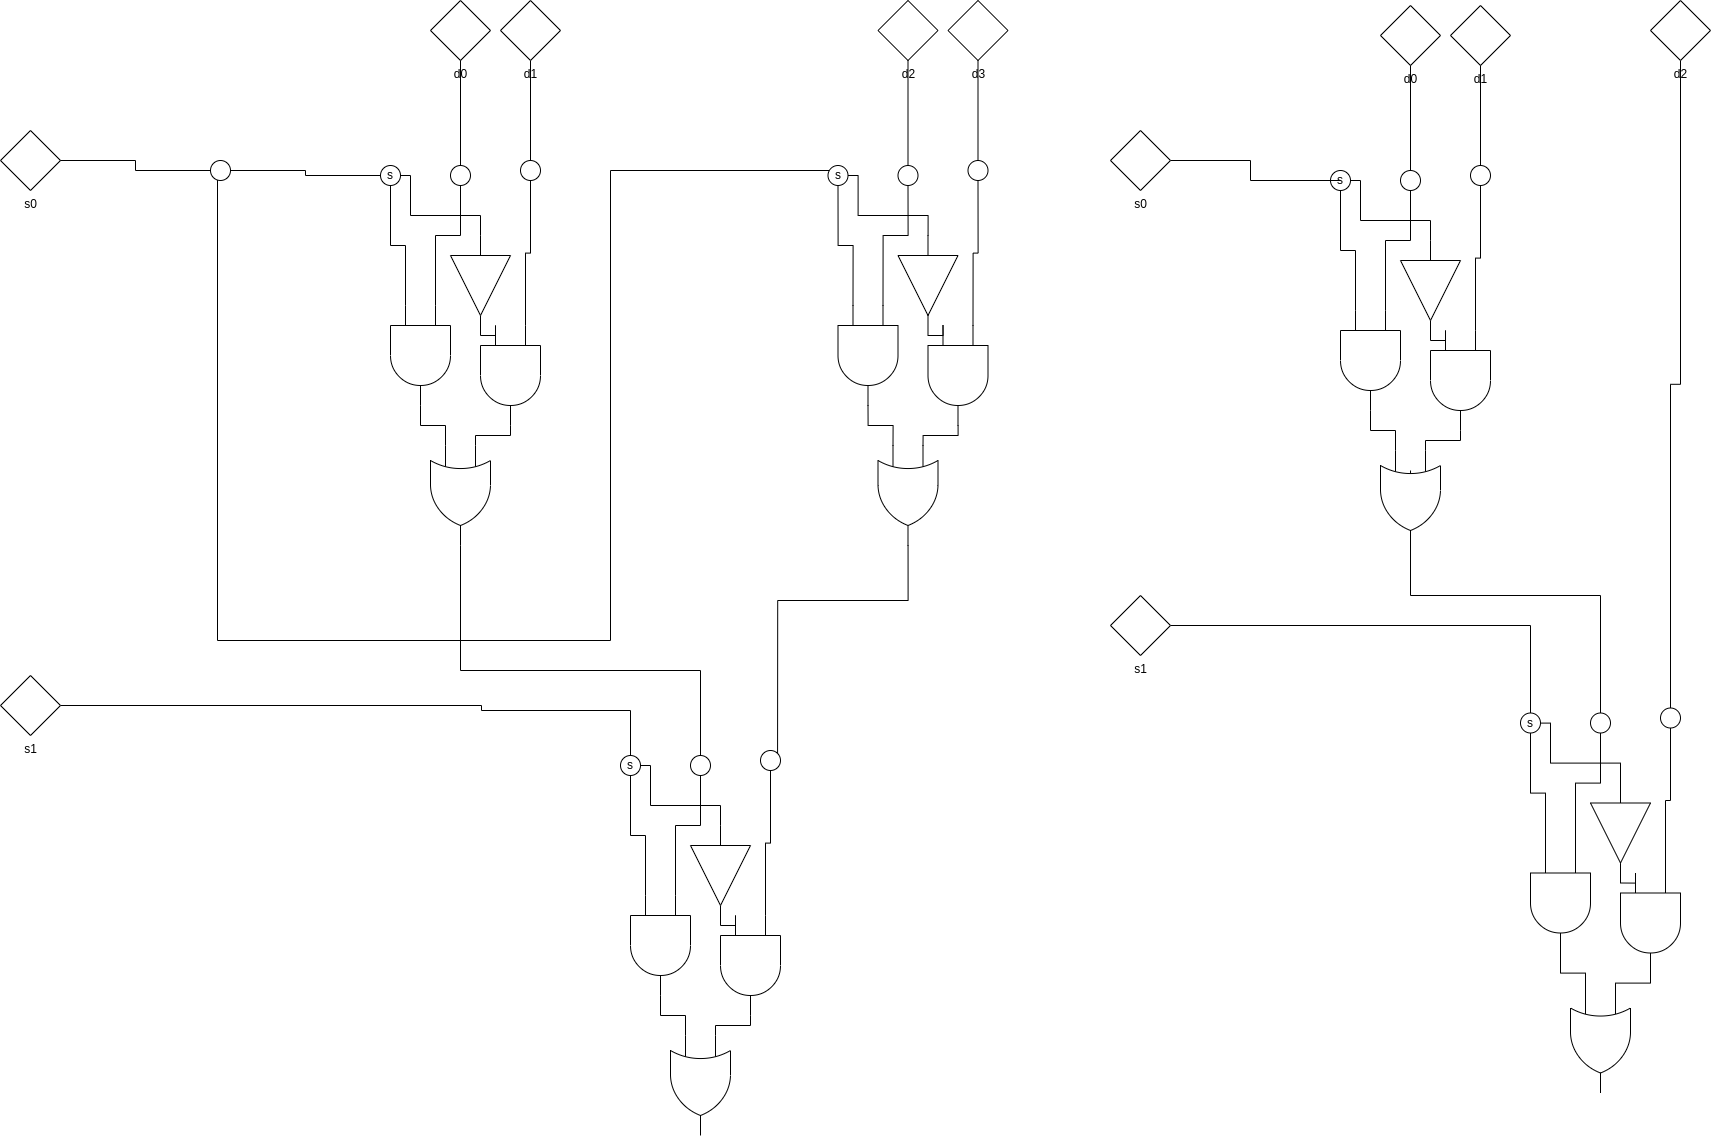
\includegraphics[height=0.6\paperheight]{./figures/3_to_1_multiplexer.png}
  %   \caption{4-to-1 and 3-to-1 Multiplexer}
  % \end{figure}
\end{frame}

\if\preview0{
\begin{frame}[allowframebreaks]{Task 1 - Memory Map}{Task 1.2\vspace{0.25cm}}
  \begin{itemize}
    \item \alert{memory cell area:}
    \begin{itemize}
      \item for a $8$-\alert{bit address}, we need $2^8$ \alert{memory cells}.
      \item $C=2^8 \cdot A_{\mathrm{mem}}=2^8 \cdot 6=1536$.
    \end{itemize}
    \item \alert{$u$-bit decoder area:}
    \begin{itemize}
      \item for activating one of the $2^u$ \alert{word lines}.
      \item we construct a $k$-bit decoder using $2$ \alert{smaller decoders} and $2^k$ $2$-input \alert{AND gates}.
      \item the \alert{smaller decoders} should be of size $\frac{k}{2}$ if $k$ is \alert{even}, or of sizes $\frac{k + 1}{2}$ and $\frac{k - 1}{2}$ if $k$ is \alert{odd}.
      \item $D(k)= \begin{cases}A_{\mathrm{NOT}} & \text { if } k=1 \\ 2 \cdot D\left(\frac{k}{2}\right)+A_{\mathrm{AND}} \cdot 2^k & \text { if } k>1 \text { and } k \text { is even } \\ D\left(\frac{k-1}{2}\right)+D\left(\frac{k+1}{2}\right)+A_{\mathrm{AND}} \cdot 2^k & \text { if } k>1 \text { and } k \text { is odd }\end{cases}$
    \end{itemize}
    \item \alert{$2w$-to-$1$ multiplexer area:}
    \begin{itemize}
      \item  for selecting one of the $2^w$ \alert{bit lines}.
      \item  we can construct a $2^k$-to-$1$ \alert{multiplexer} for any $k$ using two $2^{k-1}$-to-$1$ \alert{multiplexers} and one $2$-to-$1$ \alert{multiplexer}.
      \item $M(k)= \begin{cases}A_{\operatorname{mux}} = 4 & \text { if } k=1 \\ 2 \cdot M(k-1)+A_{\operatorname{mux}} & \text { otherwise }\end{cases}$.
    \end{itemize}
    \item \alert{single sense amplifier area:}
    \begin{itemize}
      \item for each of the $w$ \alert{column bit lines}
      \item $S(w)=2^w \cdot A_{\text {sense}}$
    \end{itemize}
    \item there are $8$ possible \alert{implementations} for $u$ and $w$
    \item the area \alert{excluding} the memory cells: D(u) + M (w) + S(w)
  \end{itemize}
\end{frame}

\begin{frame}{Task 1 - Memory Map}{Task 1.2\vspace{0.25cm}}
  \centering
 \begin{table}
   \begin{tabular}{|c|c||c|c|c|c|}
      \hline$u$ & $w$ & Decoder $D(u)$ & Multiplexer $M(w)$ & Sense Amp $S(w)$ & Total \\
      \hline \hline 0 & 8 & 0 & 1020 & 1280 & 2300 \\
      \hline 1 & 7 & 1 & 508 & 640 & 1149 \\
      \hline 2 & 6 & 6 & 252 & 320 & 578 \\
      \hline 3 & 5 & 15 & 124 & 160 & 299 \\
      \hline 4 & 4 & 28 & 60 & 80 & 168 \\
      \hline 5 & 3 & 53 & 28 & 40 & 121 \\
      \hline 6 & 2 & 94 & 12 & 20 & 126 \\
      \hline 7 & 1 & 171 & 4 & 10 & 185 \\
      \hline 8 & 0 & 312 & 0 & 5 & 317 \\
      \hline
    \end{tabular}
    \caption{Different SRAM implementations}
 \end{table}
\end{frame}
}\fi

%!Tex Root = ../Tutorat5.tex
% ./Packete.tex
% ./Design.tex
% ./Deklarationen.tex
% ./Aufgabe1.tex
% ./Aufgabe3.tex
% ./Bonus.tex

\section{Task 2}

\setcounter{task}{1}

\begin{frame}[allowframebreaks]{Task 2}{}
  \begin{tasknoinc}
    \centering
    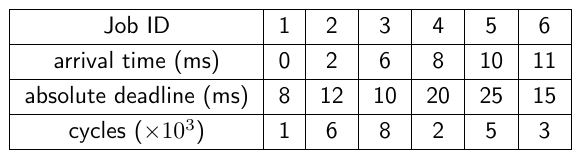
\includegraphics[width=0.8\paperheight]{./figures/task2.png}
  \end{tasknoinc}
  \begin{requirements}
    \begin{itemize}
      \item $V^{\prime}\left(\left[z, z^{\prime}\right]\right)=\left\{v_i \in V: z \leq a_i<d_i \leq z^{\prime}\right\}$
      \item $G\left(\left[z, z^{\prime}\right]\right)=\sum_{v_i \in V^{\prime}\left(\left[z, z^{\prime}\right]\right)} c_i /\left(z^{\prime}-z\right)$
    \end{itemize}
  \end{requirements}
\end{frame}

\begin{frame}[allowframebreaks]{Task 2}{}
  \begin{solutionnoinc}
    \begin{ganttchart}[
        x unit=0.4cm,
        y unit chart=0.7cm,
        canvas/.style={draw=none,fill=none}, % remove canvas borders, etc
        vgrid={*1{draw=black!12}},           % vertical gray lines every unit
        inline,                              % draw bars inline
        group/.style={draw=none,fill=none},  % remove group borders, etc
        bar top shift=0.1,                   % give bar 10% padding top/bottom
        bar height=0.8,                      % bar size 80% of vertical space
        y unit title=0.5cm,                  % crop titles a little smaller
        title/.style={draw=none,fill=none},  % remove title borders, etc
        include title in canvas=false        % no vertical grid in title
      ]{-1}{26}

      \gantttitle{0}{2}
      \gantttitle{2}{2}
      \gantttitle{4}{2}
      \gantttitle{6}{2}
      \gantttitle{8}{2}
      \gantttitle{10}{2}
      \gantttitle{12}{2}
      \gantttitle{14}{2}
      \gantttitle{16}{2}
      \gantttitle{18}{2}
      \gantttitle{20}{2}
      \gantttitle{22}{2}
      \gantttitle{24}{2}
      \gantttitle{26}{2} \\

      \ganttgroup[inline=false]{$T_{1}$}{0}{1}
      \ganttbar[bar/.style={fill=red, fill opacity=0.3}]{1 (n=1)}{0}{7}\\

      \ganttgroup[inline=false]{$T_{2}$}{0}{1}
      \ganttbar[bar/.style={fill=orange, fill opacity=0.3}]{2 (n=6)}{2}{11}\\

      \ganttgroup[inline=false]{$T_{3}$}{0}{1}
      \ganttbar[bar/.style={fill=yellow, fill opacity=0.3}]{3 (n=8)}{6}{9}\\

      \ganttgroup[inline=false]{$T_{4}$}{0}{1}
      \ganttbar[bar/.style={fill=green, fill opacity=0.3}]{4 (n=2)}{8}{19}\\

      \ganttgroup[inline=false]{$T_{5}$}{0}{1}
      \ganttbar[bar/.style={fill=blue, fill opacity=0.3}]{5 (n=5)}{10}{24}\\

      \ganttgroup[inline=false]{$T_{6}$}{0}{1}
      \ganttbar[bar/.style={fill=cyan, fill opacity=0.3}]{6 (n=3)}{11}{14}

    \end{ganttchart}
  \end{solutionnoinc}
  \begin{solutionnoinc}
    \tiny
    \begin{columns}
      \begin{column}{0.33\textwidth}
        \begin{itemize}
          \item $G([0, 8]) = \frac{1}{8} = 0.125$
          \item $G([0, 12]) = \frac{1+6+8}{12} = 1.25$
          \item $G([0, 10]) = \frac{1+8}{10} = 0.9$
          \item $G([0, 20]) = \frac{1+6+8+2+3}{20} = 1$
          \item $G([0, 25]) = \frac{1+6+8+2+3+5}{25} = 1$
          \item $G([0, 15]) = \frac{1+6+8+3}{15} = 1.2$
          \item $G([2, 12]) = \frac{6+8}{10} = 1.4$
        \end{itemize}
      \end{column}
      \begin{column}{0.33\textwidth}
        \begin{itemize}
          \item $G([2, 10]) = \frac{8}{8} = 1$
          \item $G([2, 20]) = \frac{6+8+2+3}{18} = 1.06$
          \item $G([2, 25]) = \frac{6+8+2+3+5}{23} = 1.04$
          \item $G([2, 15]) = \frac{6+8+3}{13} = 1.31$
          \item $\boxed{G([6, 10]) = \frac{8}{4} = 2}$
          \item $G([6, 20]) = \frac{8+2+3}{14} = 0.93$
          \item $G([6, 25]) = \frac{8+2+3+5}{19} = 0.95$
        \end{itemize}
      \end{column}
      \begin{column}{0.33\textwidth}
        \begin{itemize}
          \item $G([6, 15]) = \frac{8+3}{9} = 1.22$
          \item $G([8, 20]) = \frac{2+3}{12} = 0.42$
          \item $G([8, 25]) = \frac{2+3+5}{17} = 0.59$
          \item $G([8, 15]) = \frac{3}{7} = 0.43$
          \item $G([10, 25]) = \frac{5+3}{15} = 5.3$
          \item $G([10, 15]) = \frac{3}{5} = 0.6$
          \item $G([11, 15]) = \frac{3}{4} = 0.75$
        \end{itemize}
      \end{column}
    \end{columns}
  \end{solutionnoinc}
  \begin{solutionnoinc}
    \begin{ganttchart}[
        x unit=0.4cm,
        y unit chart=0.7cm,
        canvas/.style={draw=none,fill=none}, % remove canvas borders, etc
        vgrid={*1{draw=black!12}},           % vertical gray lines every unit
        inline,                              % draw bars inline
        group/.style={draw=none,fill=none},  % remove group borders, etc
        bar top shift=0.1,                   % give bar 10% padding top/bottom
        bar height=0.8,                      % bar size 80% of vertical space
        y unit title=0.5cm,                  % crop titles a little smaller
        title/.style={draw=none,fill=none},  % remove title borders, etc
        include title in canvas=false        % no vertical grid in title
      ]{-1}{22}

      \gantttitle{0}{2}
      \gantttitle{2}{2}
      \gantttitle{4}{2}
      \gantttitle{6}{2}
      \gantttitle{8}{2}
      \gantttitle{10}{2}
      \gantttitle{12}{2}
      \gantttitle{14}{2}
      \gantttitle{16}{2}
      \gantttitle{18}{2}
      \gantttitle{20}{2}
      \gantttitle{22}{2} \\

      \ganttgroup[inline=false]{$T_{1}$}{0}{1}
      \ganttbar[bar/.style={fill=red, fill opacity=0.3}]{1 (n=1)}{0}{5}\\

      \ganttgroup[inline=false]{$T_{2}$}{0}{1}
      \ganttbar[bar/.style={fill=orange, fill opacity=0.3}]{2 (n=6)}{2}{7}\\

      \ganttgroup[inline=false]{$T_{4}$}{0}{1}
      \ganttbar[bar/.style={fill=green, fill opacity=0.3}]{4 (n=2)}{6}{15}\\

      \ganttgroup[inline=false]{$T_{5}$}{0}{1}
      \ganttbar[bar/.style={fill=blue, fill opacity=0.3}]{5 (n=5)}{6}{20}\\

      \ganttgroup[inline=false]{$T_{6}$}{0}{1}
      \ganttbar[bar/.style={fill=cyan, fill opacity=0.3}]{6 (n=3)}{7}{10}
    \end{ganttchart}
  \end{solutionnoinc}
  \begin{solutionnoinc}
    \scriptsize
    \begin{columns}
      \begin{column}[t]{0.5\textwidth}
        \begin{itemize}
          \item $G([0, 6]) = \frac{1}{6} = 0.17$
          \item $G([0, 8]) = \frac{1+6}{8} = 0.875$
          \item $G([0, 16]) = \frac{1+6+2+3}{16} = 0.75$
          \item $G([0, 21]) = \frac{1+6+2+5+3}{21} = 0.81$
          \item $G([0, 11]) = \frac{1+6+3}{11} = 0.91$
          \item $G([2, 8]) = \frac{6}{6} = 1$
          \item $G([2, 16]) = \frac{6+2+3}{14} = 0.79$
          \item $G([2, 21]) = \frac{6+2+5+3}{19} = 0.84$
        \end{itemize}
      \end{column}
      \begin{column}[t]{0.5\textwidth}
        \begin{itemize}
          \item $\boxed{G([2, 11]) = \frac{6+3}{9} = 1}$
          \item $G([6, 16]) = \frac{2+3}{10} = 0.5$
          \item $G([6, 21]) = \frac{2+5+3}{15} = 0.67$
          \item $G([6, 11]) = \frac{3}{5} = 0.6$
          \item $G([7, 11]) = \frac{3}{4} = 0.75$
        \end{itemize}
      \end{column}
    \end{columns}
  \end{solutionnoinc}
  \begin{solutionnoinc}
    \begin{ganttchart}[
        x unit=0.4cm,
        y unit chart=0.7cm,
        canvas/.style={draw=none,fill=none}, % remove canvas borders, etc
        vgrid={*1{draw=black!12}},           % vertical gray lines every unit
        inline,                              % draw bars inline
        group/.style={draw=none,fill=none},  % remove group borders, etc
        bar top shift=0.1,                   % give bar 10% padding top/bottom
        bar height=0.8,                      % bar size 80% of vertical space
        y unit title=0.5cm,                  % crop titles a little smaller
        title/.style={draw=none,fill=none},  % remove title borders, etc
        include title in canvas=false        % no vertical grid in title
      ]{-1}{12}

      \gantttitle{0}{2}
      \gantttitle{2}{2}
      \gantttitle{4}{2}
      \gantttitle{6}{2}
      \gantttitle{8}{2}
      \gantttitle{10}{2}
      \gantttitle{12}{2} \\

      \ganttgroup[inline=false]{$T_{1}$}{0}{1}
      \ganttbar[bar/.style={fill=red, fill opacity=0.3}]{1 (n=1)}{0}{1}\\

      \ganttgroup[inline=false]{$T_{4}$}{0}{1}
      \ganttbar[bar/.style={fill=green, fill opacity=0.3}]{4 (n=2)}{2}{6}\\

      \ganttgroup[inline=false]{$T_{5}$}{0}{1}
      \ganttbar[bar/.style={fill=blue, fill opacity=0.3}]{5 (n=5)}{2}{11}\\
    \end{ganttchart}
  \end{solutionnoinc}
  \begin{solutionnoinc}
    \begin{itemize}
      \item $G([0, 2]) = \frac{1}{2} = 0.5$
      \item $G([0, 7]) = \frac{1+2}{7} = 0.43$
      \item $G([0, 12]) = \frac{1+2+5}{12} = 0.67$
      \item $G([2, 7]) = \frac{2}{5} = 0.4$
      \item $\boxed{G([2, 12]) = \frac{2+5}{10} = 0.7}$
    \end{itemize}
  \end{solutionnoinc}
  \begin{solutionnoinc}
    \begin{ganttchart}[
        x unit=0.4cm,
        y unit chart=0.7cm,
        canvas/.style={draw=none,fill=none}, % remove canvas borders, etc
        vgrid={*1{draw=black!12}},           % vertical gray lines every unit
        inline,                              % draw bars inline
        group/.style={draw=none,fill=none},  % remove group borders, etc
        bar top shift=0.1,                   % give bar 10% padding top/bottom
        bar height=0.8,                      % bar size 80% of vertical space
        y unit title=0.5cm,                  % crop titles a little smaller
        title/.style={draw=none,fill=none},  % remove title borders, etc
        include title in canvas=false        % no vertical grid in title
      ]{-1}{2}

      \gantttitle{0}{2}
      \gantttitle{2}{2} \\

      \ganttgroup[inline=false]{$T_{1}$}{0}{1}
      \ganttbar[bar/.style={fill=red, fill opacity=0.3}]{1 (n=1)}{0}{1}\\
    \end{ganttchart}
  \begin{itemize}
    \item $\boxed{G([0, 2]) = \frac{1}{2} = 0.5}$
  \end{itemize}
  \end{solutionnoinc}
\end{frame}

\begin{frame}[allowframebreaks]{Task 2}{}
  \begin{solution}
    \begin{tikzpicture}
      \begin{axis}[x=0.4cm, y=2cm, xtick={0, 2, ..., 25}, ytick={0, 0.5, ...,2}, axis lines=left,
        ymajorgrids=true, ymin=0, xlabel=$time (ms)$, xlabel style={at={(0.4,-0.1)}, anchor=west},
        ylabel=$frequency (1 MHz)$, ylabel style={rotate=-90,at={(0.1,1)}, anchor=south}
        ]
      \addplot [
        ybar interval,
        xtick=data,
        x tick label style={
        rotate=90,
        anchor=east,
        },
        color=red, fill=red, fill opacity=0.3
      ] coordinates {
        (0,0.5) (2,0.5)
      };
      \addplot [
        ybar interval,
        xtick=data,
        x tick label style={
        rotate=90,
        anchor=east,
        },
        color=orange, fill=orange, fill opacity=0.3
      ] coordinates {
        (2,1) (6,1)
      };
      \addplot [
        ybar interval,
        xtick=data,
        x tick label style={
        rotate=90,
        anchor=east,
        },
        color=yellow, fill=yellow, fill opacity=0.3
      ] coordinates {
        (6,2) (10,2)
      };
      \addplot [
        ybar interval,
        xtick=data,
        x tick label style={
        rotate=90,
        anchor=east,
        },
        color=orange, fill=orange, fill opacity=0.3
      ] coordinates {
        (10,1) (12,1)
      };
      \addplot [
        ybar interval,
        xtick=data,
        x tick label style={
        rotate=90,
        anchor=east,
        },
        color=cyan, fill=cyan, fill opacity=0.3
      ] coordinates {
        (12,1) (15,1)
      };
      \addplot [
        ybar interval,
        xtick=data,
        x tick label style={
        rotate=90,
        anchor=east,
        },
        color=green, fill=green, fill opacity=0.3
      ] coordinates {
        (15,0.7) (18,.07)
      };
      \addplot [
        ybar interval,
        xtick=data,
        x tick label style={
        rotate=90,
        anchor=east,
        },
        color=blue, fill=blue, fill opacity=0.3
      ] coordinates {
        (18,0.7) (25,0.7)
      };
    \end{axis}
    \end{tikzpicture}
  \end{solution}
\end{frame}

\begin{frame}[allowframebreaks]{Task 2}{}
  \begin{solutionnoinc}
    \begin{ganttchart}[
        x unit=0.4cm,
        y unit chart=0.7cm,
        canvas/.style={draw=none,fill=none}, % remove canvas borders, etc
        vgrid={*1{draw=black!12}},           % vertical gray lines every unit
        inline,                              % draw bars inline
        group/.style={draw=none,fill=none},  % remove group borders, etc
        bar top shift=0.1,                   % give bar 10% padding top/bottom
        bar height=0.8,                      % bar size 80% of vertical space
        y unit title=0.5cm,                  % crop titles a little smaller
        title/.style={draw=none,fill=none},  % remove title borders, etc
        include title in canvas=false        % no vertical grid in title
      ]{-1}{26}

      \gantttitle{0}{2}
      \gantttitle{2}{2}
      \gantttitle{4}{2}
      \gantttitle{6}{2}
      \gantttitle{8}{2}
      \gantttitle{10}{2}
      \gantttitle{12}{2}
      \gantttitle{14}{2}
      \gantttitle{16}{2}
      \gantttitle{18}{2}
      \gantttitle{20}{2}
      \gantttitle{22}{2}
      \gantttitle{24}{2}
      \gantttitle{26}{2} \\

      \ganttgroup[inline=false]{$T_{1}$}{0}{1}
      \ganttbar[bar/.style={fill=red, fill opacity=0.3}]{1 (n=1)}{0}{7}\\

      \ganttgroup[inline=false]{$T_{2}$}{0}{1}
      \ganttbar[bar/.style={fill=orange, fill opacity=0.3}]{2 (n=6)}{2}{11}\\

      \ganttgroup[inline=false]{$T_{3}$}{0}{1}
      \ganttbar[bar/.style={fill=yellow, fill opacity=0.3}]{3 (n=8)}{6}{9}\\

      \ganttgroup[inline=false]{$T_{4}$}{0}{1}
      \ganttbar[bar/.style={fill=green, fill opacity=0.3}]{4 (n=2)}{8}{19}\\

      \ganttgroup[inline=false]{$T_{5}$}{0}{1}
      \ganttbar[bar/.style={fill=blue, fill opacity=0.3}]{5 (n=5)}{10}{24}\\

      \ganttgroup[inline=false]{$T_{6}$}{0}{1}
      \ganttbar[bar/.style={fill=cyan, fill opacity=0.3}]{6 (n=3)}{11}{14}
    \end{ganttchart}
  \end{solutionnoinc}
  \begin{solutionnoinc}
    \begin{itemize}
      \item $\boxed{G([0, 8]) = \frac{1}{8} = 0.125}$
    \end{itemize}
  \end{solutionnoinc}
  \framebreak
  \begin{solutionnoinc}
    \begin{ganttchart}[
        x unit=0.4cm,
        y unit chart=0.7cm,
        canvas/.style={draw=none,fill=none}, % remove canvas borders, etc
        vgrid={*1{draw=black!12}},           % vertical gray lines every unit
        inline,                              % draw bars inline
        group/.style={draw=none,fill=none},  % remove group borders, etc
        bar top shift=0.1,                   % give bar 10% padding top/bottom
        bar height=0.8,                      % bar size 80% of vertical space
        y unit title=0.5cm,                  % crop titles a little smaller
        title/.style={draw=none,fill=none},  % remove title borders, etc
        include title in canvas=false        % no vertical grid in title
      ]{-1}{8}

      \gantttitle{0}{2}
      \gantttitle{2}{2}
      \gantttitle{4}{2}
      \gantttitle{6}{2}
      \gantttitle{8}{2}
      \gantttitle{10}{2}
      \gantttitle{12}{2}
      \gantttitle{14}{2}
      \gantttitle{16}{2}
      \gantttitle{18}{2}
      \gantttitle{20}{2} \\

      \ganttgroup[inline=false]{$T_{1}$}{0}{1}
      \ganttbar[bar/.style={fill=red, fill opacity=0.3}]{1 (n=0.75)}{2}{7}\\

      \ganttgroup[inline=false]{$T_{2}$}{0}{1}
      \ganttbar[bar/.style={fill=orange, fill opacity=0.3}]{2 (n=6)}{2}{11}\\
    \end{ganttchart}
  \end{solutionnoinc}
  \framebreak
  \begin{solutionnoinc}
    \begin{itemize}
      \item $G([2, 8]) = \frac{1-0.125\cdot 2}{6} = 0.125$
      \item $\boxed{G([2, 12]) = \frac{(1-0.125\cdot 2) + 6}{10} = 0.675}$
      \item $d_1 = 8 > 12 = d_2$, Task 1 has ealier dealine (EDF)
      \item $\displaystyle T_1 = \frac{0.75}{0.675} \approx 1.11, d_1^* = 2 + 1.11 = 3.11$
    \end{itemize}
  \end{solutionnoinc}
  \framebreak
  \begin{solutionnoinc}
    \begin{ganttchart}[
        x unit=0.4cm,
        y unit chart=0.7cm,
        canvas/.style={draw=none,fill=none}, % remove canvas borders, etc
        vgrid={*1{draw=black!12}},           % vertical gray lines every unit
        inline,                              % draw bars inline
        group/.style={draw=none,fill=none},  % remove group borders, etc
        bar top shift=0.1,                   % give bar 10% padding top/bottom
        bar height=0.8,                      % bar size 80% of vertical space
        y unit title=0.5cm,                  % crop titles a little smaller
        title/.style={draw=none,fill=none},  % remove title borders, etc
        include title in canvas=false        % no vertical grid in title
      ]{-1}{12}

      \gantttitle{0}{2}
      \gantttitle{2}{2}
      \gantttitle{4}{2}
      \gantttitle{6}{2}
      \gantttitle{8}{2}
      \gantttitle{10}{2}
      \gantttitle{12}{2} \\

      \ganttgroup[inline=false]{$T_{2}$}{0}{1}
      \ganttbar[bar/.style={fill=orange, fill opacity=0.3}]{2 (n=4.05)}{6}{11}\\

      \ganttgroup[inline=false]{$T_{3}$}{0}{1}
      \ganttbar[bar/.style={fill=yellow, fill opacity=0.3}]{3 (n=8)}{6}{9}\\
    \end{ganttchart}
  \end{solutionnoinc}
  \framebreak
  \begin{solutionnoinc}
    \begin{itemize}
      \item $G([6, 10]) = \frac{6 - (0.675 \cdot (4 - 1.111))}{4} = 1.01$
      \item $\boxed{G([6, 12]) = \frac{6 - (0.675 \cdot (4 - 1.111)) + 8}{6} = 2.01}$
      \item $d_2 = 12 > 10 = d_3$, Task 3 has ealier dealine (EDF)
      \item $T_3=\frac{8}{2.01} \approx 3.98, d_3^* = 6 + 3.98 \approx 10$
      % \item $T_2=\frac{4.05}{2.01} \approx 2.01, d_2^* = 6 + 2.01 \approx 10$
    \end{itemize}
  \end{solutionnoinc}
  \framebreak
  \begin{solutionnoinc}
    \begin{ganttchart}[
        x unit=0.4cm,
        y unit chart=0.7cm,
        canvas/.style={draw=none,fill=none}, % remove canvas borders, etc
        vgrid={*1{draw=black!12}},           % vertical gray lines every unit
        inline,                              % draw bars inline
        group/.style={draw=none,fill=none},  % remove group borders, etc
        bar top shift=0.1,                   % give bar 10% padding top/bottom
        bar height=0.8,                      % bar size 80% of vertical space
        y unit title=0.5cm,                  % crop titles a little smaller
        title/.style={draw=none,fill=none},  % remove title borders, etc
        include title in canvas=false        % no vertical grid in title
      ]{-1}{20}

      \gantttitle{0}{2}
      \gantttitle{2}{2}
      \gantttitle{4}{2}
      \gantttitle{6}{2}
      \gantttitle{8}{2}
      \gantttitle{10}{2}
      \gantttitle{12}{2}
      \gantttitle{14}{2}
      \gantttitle{16}{2}
      \gantttitle{18}{2}
      \gantttitle{20}{2}\\

      \ganttgroup[inline=false]{$T_{2+3}$}{0}{1}
      \ganttbar[bar/.style={fill=yellow, fill opacity=0.3}]{\qquad 2+3 (n=2.01)}{8}{9}
      \ganttbar[bar/.style={fill=orange, fill opacity=0.3}]{}{10}{11}\\

      \ganttgroup[inline=false]{$T_{4}$}{0}{1}
      \ganttbar[bar/.style={fill=green, fill opacity=0.3}]{4 (n=2)}{8}{19}\\
    \end{ganttchart}
  \end{solutionnoinc}
  \framebreak
  \begin{solutionnoinc}
    \begin{itemize}
      \item $G([8, 10]) = \frac{8-2.01 \cdot 2}{2} \approx 1.99$
      \item $\boxed{G([8, 12]) = \frac{6-0.675 \cdot (4-1.111) + 8-2.01 \cdot 2}{4} \approx 2.01}$
      \item $G([8, 20]) = \frac{6-0.675 \cdot (4-1.111) + 8-2.01 \cdot 2 + 2}{12} \approx 0.84$
    \end{itemize}
  \end{solutionnoinc}
  \framebreak
  \begin{solutionnoinc}
    \begin{ganttchart}[
        x unit=0.4cm,
        y unit chart=0.7cm,
        canvas/.style={draw=none,fill=none}, % remove canvas borders, etc
        vgrid={*1{draw=black!12}},           % vertical gray lines every unit
        inline,                              % draw bars inline
        group/.style={draw=none,fill=none},  % remove group borders, etc
        bar top shift=0.1,                   % give bar 10% padding top/bottom
        bar height=0.8,                      % bar size 80% of vertical space
        y unit title=0.5cm,                  % crop titles a little smaller
        title/.style={draw=none,fill=none},  % remove title borders, etc
        include title in canvas=false        % no vertical grid in title
      ]{-1}{26}

      \gantttitle{0}{2}
      \gantttitle{2}{2}
      \gantttitle{4}{2}
      \gantttitle{6}{2}
      \gantttitle{8}{2}
      \gantttitle{10}{2}
      \gantttitle{12}{2}
      \gantttitle{14}{2}
      \gantttitle{16}{2}
      \gantttitle{18}{2}
      \gantttitle{20}{2}
      \gantttitle{22}{2}
      \gantttitle{24}{2}
      \gantttitle{26}{2} \\

      \ganttgroup[inline=false]{$T_{3}$}{0}{1}
      \ganttbar[bar/.style={fill=orange, fill opacity=0.3}]{3 (n=2.01)}{10}{11}\\

      \ganttgroup[inline=false]{$T_{4}$}{0}{1}
      \ganttbar[bar/.style={fill=green, fill opacity=0.3}]{4 (n=2)}{10}{19}\\

      \ganttgroup[inline=false]{$T_{5}$}{0}{1}
      \ganttbar[bar/.style={fill=blue, fill opacity=0.3}]{5 (n=5)}{10}{24}\\
    \end{ganttchart}
  \end{solutionnoinc}
  \framebreak
  \begin{solutionnoinc}
    \begin{itemize}
      \item $\boxed{G([10, 12]) = \frac{6-0.675 \cdot (4-1.111)}{2} \approx 2.02}$ (rounding error)
      \item $G([10, 20]) = \frac{6-0.675 \cdot (4-1.111) + 2}{10} \approx 0.6$
      \item $G([10, 25]) = \frac{6-0.675 \cdot (4-1.111) + 2 + 5}{15} \approx 0.74$
    \end{itemize}
  \end{solutionnoinc}
  \framebreak
  \begin{solutionnoinc}
    \begin{ganttchart}[
        x unit=0.4cm,
        y unit chart=0.7cm,
        canvas/.style={draw=none,fill=none}, % remove canvas borders, etc
        vgrid={*1{draw=black!12}},           % vertical gray lines every unit
        inline,                              % draw bars inline
        group/.style={draw=none,fill=none},  % remove group borders, etc
        bar top shift=0.1,                   % give bar 10% padding top/bottom
        bar height=0.8,                      % bar size 80% of vertical space
        y unit title=0.5cm,                  % crop titles a little smaller
        title/.style={draw=none,fill=none},  % remove title borders, etc
        include title in canvas=false        % no vertical grid in title
      ]{-1}{26}

      \gantttitle{0}{2}
      \gantttitle{2}{2}
      \gantttitle{4}{2}
      \gantttitle{6}{2}
      \gantttitle{8}{2}
      \gantttitle{10}{2}
      \gantttitle{12}{2}
      \gantttitle{14}{2}
      \gantttitle{16}{2}
      \gantttitle{18}{2}
      \gantttitle{20}{2}
      \gantttitle{22}{2}
      \gantttitle{24}{2}
      \gantttitle{26}{2} \\

      \ganttgroup[inline=false]{$T_{3}$}{0}{1}
      \ganttbar[bar/.style={fill=orange, fill opacity=0.3}]{3 (n=2.01)}{11}{11}\\

      \ganttgroup[inline=false]{$T_{4}$}{0}{1}
      \ganttbar[bar/.style={fill=green, fill opacity=0.3}]{4 (n=2)}{11}{19}\\

      \ganttgroup[inline=false]{$T_{5}$}{0}{1}
      \ganttbar[bar/.style={fill=blue, fill opacity=0.3}]{5 (n=5)}{11}{24}\\

      \ganttgroup[inline=false]{$T_{6}$}{0}{1}
      \ganttbar[bar/.style={fill=cyan, fill opacity=0.3}]{6 (n=6)}{11}{14}\\
    \end{ganttchart}
  \end{solutionnoinc}
  \framebreak
  \begin{solutionnoinc}
    \begin{itemize}
      \item $\boxed{G([11, 12]) = \frac{6-0.675 \cdot (4-1.111) - 1 \cdot 2.01}{1} \approx 2.04}$ (rounding error)
      \item $G([11, 15]) = \frac{6-0.675 \cdot (4-1.111) - 1 \cdot 2.01 + 3}{4} \approx 1.26$
      \item $G([11, 20]) = \frac{6-0.675 \cdot (4-1.111) - 1 \cdot 2.01 + 3 + 2}{9} \approx 0.78$
      \item $G([11, 25]) = \frac{6-0.675 \cdot (4-1.111) - 1 \cdot 2.01 + 3 + 5 + 2}{14} \approx 0.86$
    \end{itemize}
  \end{solutionnoinc}
  \begin{solutionnoinc}
    \begin{ganttchart}[
        x unit=0.4cm,
        y unit chart=0.7cm,
        canvas/.style={draw=none,fill=none}, % remove canvas borders, etc
        vgrid={*1{draw=black!12}},           % vertical gray lines every unit
        inline,                              % draw bars inline
        group/.style={draw=none,fill=none},  % remove group borders, etc
        bar top shift=0.1,                   % give bar 10% padding top/bottom
        bar height=0.8,                      % bar size 80% of vertical space
        y unit title=0.5cm,                  % crop titles a little smaller
        title/.style={draw=none,fill=none},  % remove title borders, etc
        include title in canvas=false        % no vertical grid in title
      ]{-1}{26}

      \gantttitle{0}{2}
      \gantttitle{2}{2}
      \gantttitle{4}{2}
      \gantttitle{6}{2}
      \gantttitle{8}{2}
      \gantttitle{10}{2}
      \gantttitle{12}{2}
      \gantttitle{14}{2}
      \gantttitle{16}{2}
      \gantttitle{18}{2}
      \gantttitle{20}{2}
      \gantttitle{22}{2}
      \gantttitle{24}{2}
      \gantttitle{26}{2} \\

      \ganttgroup[inline=false]{$T_{4}$}{0}{1}
      \ganttbar[bar/.style={fill=green, fill opacity=0.3}]{4 (n=2)}{12}{19}\\

      \ganttgroup[inline=false]{$T_{5}$}{0}{1}
      \ganttbar[bar/.style={fill=blue, fill opacity=0.3}]{5 (n=5)}{12}{24}\\

      \ganttgroup[inline=false]{$T_{6}$}{0}{1}
      \ganttbar[bar/.style={fill=cyan, fill opacity=0.3}]{6 (n=6)}{12}{14}\\
    \end{ganttchart}
  \end{solutionnoinc}
  \framebreak
  \begin{solutionnoinc}
    \begin{itemize}
      \item $\boxed{G([12, 15]) = \frac{3}{3} \approx 1}$
      \item $G([12, 20]) = \frac{3 + 2}{8} \approx 0.63$
      \item $G([12, 25]) = \frac{3 + 2 + 5}{13} \approx 0.62$
    \end{itemize}
  \end{solutionnoinc}
  \framebreak
  \begin{solutionnoinc}
    \begin{ganttchart}[
        x unit=0.4cm,
        y unit chart=0.7cm,
        canvas/.style={draw=none,fill=none}, % remove canvas borders, etc
        vgrid={*1{draw=black!12}},           % vertical gray lines every unit
        inline,                              % draw bars inline
        group/.style={draw=none,fill=none},  % remove group borders, etc
        bar top shift=0.1,                   % give bar 10% padding top/bottom
        bar height=0.8,                      % bar size 80% of vertical space
        y unit title=0.5cm,                  % crop titles a little smaller
        title/.style={draw=none,fill=none},  % remove title borders, etc
        include title in canvas=false        % no vertical grid in title
      ]{-1}{26}

      \gantttitle{0}{2}
      \gantttitle{2}{2}
      \gantttitle{4}{2}
      \gantttitle{6}{2}
      \gantttitle{8}{2}
      \gantttitle{10}{2}
      \gantttitle{12}{2}
      \gantttitle{14}{2}
      \gantttitle{16}{2}
      \gantttitle{18}{2}
      \gantttitle{20}{2}
      \gantttitle{22}{2}
      \gantttitle{24}{2}
      \gantttitle{26}{2} \\

      \ganttgroup[inline=false]{$T_{4}$}{0}{1}
      \ganttbar[bar/.style={fill=green, fill opacity=0.3}]{4 (n=2)}{15}{19}\\

      \ganttgroup[inline=false]{$T_{5}$}{0}{1}
      \ganttbar[bar/.style={fill=blue, fill opacity=0.3}]{5 (n=5)}{15}{24}\\
    \end{ganttchart}
  \end{solutionnoinc}
  \framebreak
  \begin{solutionnoinc}
    \begin{itemize}
      \item $G([15, 20]) = \frac{2}{5} \approx 0.4$
      \item $\boxed{G([15, 25]) = \frac{2+5}{10} \approx 0.7}$
      \item $d_4 = 20 < 25 = d_5$, Task 4 has ealier dealine (EDF)
    \end{itemize}
  \end{solutionnoinc}
  \framebreak
  \begin{solutionnoinc}
    \begin{tikzpicture}
      \begin{axis}[x=0.4cm, y=2cm, xtick={0, 2, ..., 25}, ytick={0, 0.5, ...,2}, axis lines=left,
        ymajorgrids=true, ymin=0, xlabel=$time (ms)$, xlabel style={at={(0.4,-0.1)}, anchor=west},
        ylabel=$frequency (1 MHz)$, ylabel style={rotate=-90,at={(0.1,1)}, anchor=south}
        ]
      \addplot [
        ybar interval,
        xtick=data,
        x tick label style={
        rotate=90,
        anchor=east,
        },
        color=red, fill=red, fill opacity=0.3
      ] coordinates {
        (0,0.125) (2,0.675) (3.2,0.675)
      };
      \addplot [
        ybar interval,
        xtick=data,
        x tick label style={
        rotate=90,
        anchor=east,
        },
        color=orange, fill=orange, fill opacity=0.3
      ] coordinates {
        (3.2,0.675) (6,0.675)
      };
      \addplot [
        ybar interval,
        xtick=data,
        x tick label style={
        rotate=90,
        anchor=east,
        },
        color=yellow, fill=yellow, fill opacity=0.3
      ] coordinates {
        (6,2.0083) (9.983,2.0083)
      };
      \addplot [
        ybar interval,
        xtick=data,
        x tick label style={
        rotate=90,
        anchor=east,
        },
        color=orange, fill=orange, fill opacity=0.3
      ] coordinates {
        (9.983,2.0083) (12,2.0083)
      };
      \addplot [
        ybar interval,
        xtick=data,
        x tick label style={
        rotate=90,
        anchor=east,
        },
        color=cyan, fill=cyan, fill opacity=0.3
      ] coordinates {
        (12,1) (15,1)
      };
      \addplot [
        ybar interval,
        xtick=data,
        x tick label style={
        rotate=90,
        anchor=east,
        },
        color=green, fill=green, fill opacity=0.3
      ] coordinates {
        (15,0.7) (18,0.7)
      };
      \addplot [
        ybar interval,
        xtick=data,
        x tick label style={
        rotate=90,
        anchor=east,
        },
        color=blue, fill=blue, fill opacity=0.3
      ] coordinates {
        (18,0.7) (25,0.7)
      };
    \end{axis}
    \end{tikzpicture}
  \end{solutionnoinc}
\end{frame}

%!Tex Root = ../Tutorat6.tex
% ./Packete.tex
% ./Design.tex
% ./Deklarationen.tex
% ./Aufgabe1.tex
% ./Aufgabe2.tex
% ./Bonus.tex

\section{Task 3}

\setcounter{task}{1}

\begin{frame}{Task 3}{Application control}
    \begin{tasknoinc}
        Consider the energy harvesting profile p(t) given in Figure 4 that repeats daily. What is the maximum average power $u_{max}$ that can be used by the system?
    \end{tasknoinc}
\end{frame}

\begin{frame}{Task 3}{Application control}
    \begin{solutionnoinc}
        \begin{figure}
            \centering
            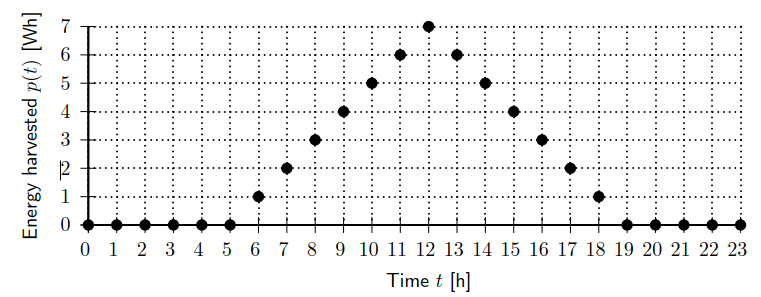
\includegraphics[scale=0.5]{figures/harvestingProfile.PNG}
        \end{figure}
    \end{solutionnoinc}
\end{frame}

\begin{frame}{Task 3}{Application control}
    \begin{solution}
        \begin{itemize}
            \item The daily harvested energy is calculated by: $(1Wh + 2Wh + 3Wh + 4Wh + 5H + 6Wh) * 2 + 7 Wh = 49Wh$
            \item This results in the following maximum average harvesting power: $u_{max} = \frac{49 Wh}{24h} = 2.04W$
        \end{itemize}
    \end{solution}
\end{frame}
\begin{frame}{Task 3}{Application control}
    \begin{tasknoinc}
        Given the knowledge of the daily energy input profile $p(t)$ in Figure 5, calculate the minimal battery size $B_{min}$ such that the used energy satisfies $u(t) = 2$ for every time interval during a day. Complete the diagram in Figure 6 with the daily evolution of the used energy $u(t)$ and the battery charge state $b(t)$ at the beginning of the interval for the found battery size $B_min$.
    \end{tasknoinc}
\end{frame}
\begin{frame}{Task 3}{Application control}
    \begin{solutionnoinc}
        \begin{itemize}
            \item The energy used during night, where the harvested energy is \alert{lower} than the consumed energy, is: $1Wh + 11 \cdot 2Wh + 1Wh = 24Wh$
            \item We need at least this much energy in our battery to compensate this deficit, meaning $B \geq 24Wh \Rightarrow B_{min} = 24Wh$.
        \end{itemize}
    \end{solutionnoinc}
\end{frame}
\begin{frame}[allowframebreaks]{Task 3}{Application control}
  \begin{figure}
      \centering
      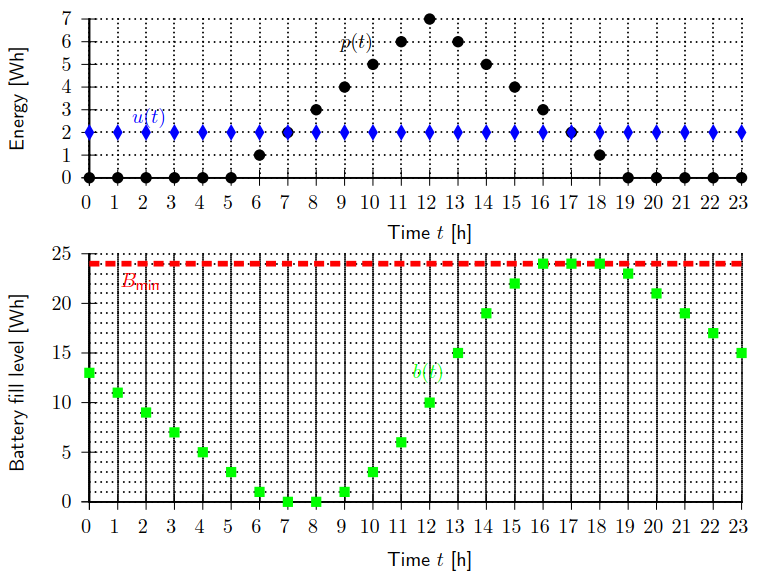
\includegraphics[scale=0.4]{figures/energyUsage.PNG}
  \end{figure}
  \begin{Sidenote}
    \begin{itemize}
      \item We observe that in intervals $t \in[0,6]$ and $t \in[18,23]$ of a day $u(t)>p(t)$ and therefore energy is used from the battery. In intervals $t \in[7,17]$ the battery is not used and the extra input power of intervals $t \in[8,16]$ is stored to the battery, with the battery overflowing in interval $t=16$.
    \end{itemize}
  \end{Sidenote}
\end{frame}

% %!Tex Root = ../Tutorat3.tex
% ./Packete.tex
% ./Design.tex
% ./Deklarationen.tex
% ./Aufgabe1.tex
% ./Aufgabe2.tex
% ./Aufgabe3.tex
% ./Bonus.tex

\section{Task 4}

\setcounter{task}{1}

\begin{frame}{Task 4}{EDF*}
\begin{itemize}
    \item EDF* is an alternative version of the EDF Algorithmus
    \item EDF* helps us to schedule Tasks with arbitrary arrival times \alert{\underline{and precedences}}. (contrary to EDF)
    \item EDF* manages this in polynomial time!
\end{itemize}
\end{frame}

\begin{frame}[allowframebreaks]{Task 4}{EDF* - Transformation}
\begin{itemize}
    \item EDF* transforms the arrival time and deadline of every task in the following way::
    \item[] \alert{Deadline}: \begin{enumerate}
        \item Task must finish the execution time within its deadline: $f_i \leq d_i$
        \item Task must not finish the execution time later than the maximum start time of its successor(s): $f_i \leq d_j - C_j$
        \item[$\rightarrow$] $d_i^* = min(d_i, min(d_j^* - C_j : J_i \rightarrow J_j))$
    \end{enumerate}
    \framebreak
    \item[] \alert{Arrival time} \begin{enumerate}
        \item Task must start the execution not earlier than its release time: $s_i \geq r_i$
        \item Task must not start execution earlier than the minimum finishing time of its predecessor(s): $s_i \geq r_j + C_j$
        \item[$\rightarrow$] $r_j^* = max(r_j, max(r_i^* + C_i : J_i \rightarrow J_j))$
    \end{enumerate}
\end{itemize}
\end{frame}

\begin{frame}[allowframebreaks]{Task 4}{EDF* - Example}
Given tasks $A, B, C, D, E, F, G$ with precedences $A \rightarrow C$, $B \rightarrow C$, $C \rightarrow E$, $D \rightarrow F$, $B \rightarrow D$, $C \rightarrow F$, $D \rightarrow G$.

All tasks arrive at time $t_0 = 0$, have a common deadline $d = 20$ and the following execution times:
\begin{center}
\begin{tabular}{|c|c|c|c|c|c|c|c|c|}
     \hline
     & A & B & C & D & E & F & G\\
     \hline
     \hline
     & 3 & 2 & 4 & 3 & 2 & 5 & 1\\
     \hline
\end{tabular}
\end{center}
We will now prepare the tasks for EDF*
\end{frame}

\begin{frame}{Task 4}{EDF* - Precedence graph example}
Given the precedences $A \rightarrow C$, $B \rightarrow C$, $C \rightarrow E$, $D \rightarrow F$, $B \rightarrow D$, $C \rightarrow F$, $D \rightarrow G$ we first draw the precedence graph:
\end{frame}

\begin{frame}{Task 4}{EDF* - Precedence graph example}
\begin{figure}
    \centering
    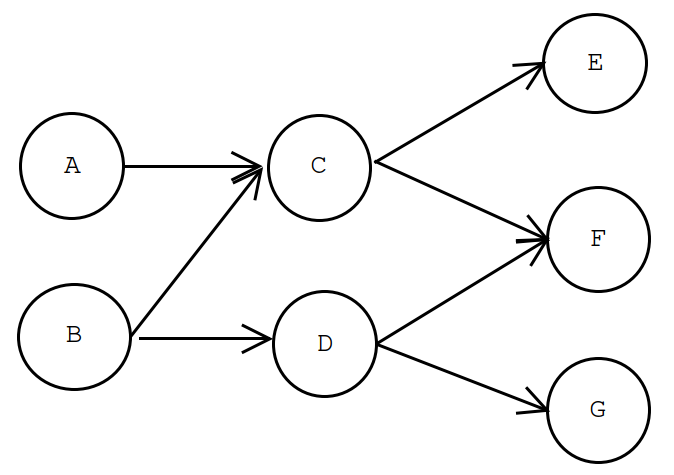
\includegraphics[scale=0.4]{figures/precedencegraph}
    \caption{Task 4: precedence graph}
    \label{pregraph}
\end{figure}
\end{frame}

\begin{frame}[allowframebreaks]{Task 4}{EDF* - Transformation example}
    \begin{itemize}
        \item $r_A^* = r_A$, $r_B^* = r_B$
        \item $r_C^* = \max\{r_C,\max\{r_A^* + C_A, r_B^* + C_B\}\} = \max\{0, \max\{3, 2\}\} = 3$
        \item $r_D^* = \max\{r_D,r_B^* + C_B\} = \max\{0, 2\} = 2$
        \item $r_F^* = \max\{r_F,\max\{r_C^* + C_C, r_D^* + C_D\}\} = \max\{0, \max\{7, 5\}\} = 7$
        \item $r_E^* = \max\{r_E,r_C^* + C_C\} = \max\{0, 7\} = 7$
        \item $r_G^* = \max\{r_G,r_D^* + C_D\} = \max\{0, 5\} = 5$
    \end{itemize}
    \framebreak
    \begin{itemize}
        \item $d_E^* = d_F^* = d_G^* = 20$
        \item $d_C^* = \min\{d_C, \min\{d_E^* - C_E, d_F^* - C_F\}\} = \min\{20, \min\{18, 15\}\} = 15$
        \item $d_D^* = 15$
        \item $d_A^* = 11$
        \item $d_B^* = 11$
    \end{itemize}
    We now successfully have transformed the problem into one without precedence and can simply use EDF!
\end{frame}
\begin{frame}{Task 4}{EDF* - Schedule}
    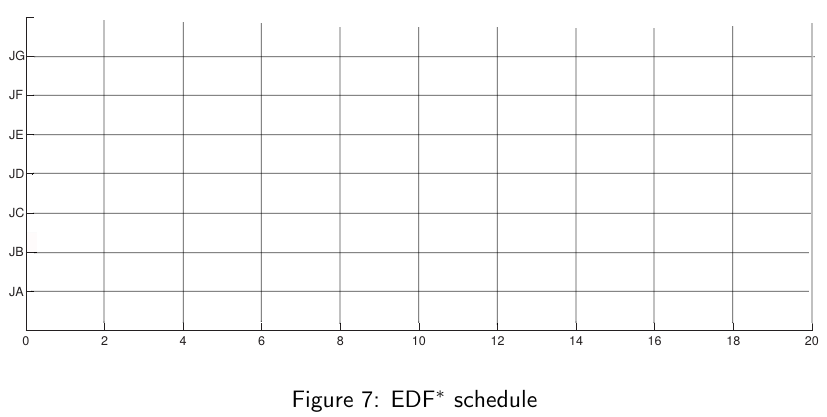
\includegraphics[width = 0.9\linewidth]{figures/EDF-star-schedule.png}
\end{frame}

\begin{frame}{Task 4}{EDF* - Schedule}
    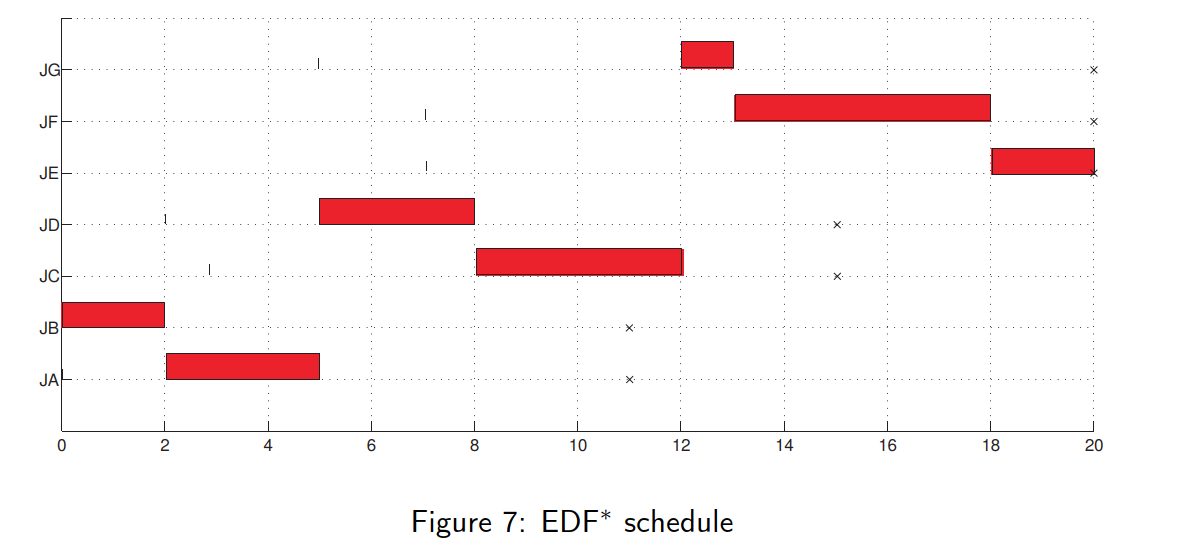
\includegraphics[width = \linewidth]{figures/edf-star-schedule-2.PNG}
\end{frame}

%!Tex Root = ../Tutorat1.tex
% ./Packete.tex
% ./Design.tex
% ./Deklarationen.tex
% ./Aufgabe1.tex
% ./Aufgabe2.tex
% ./Bonus.tex

\section{Bonus}

\begin{frame}[fragile,allowframebreaks]{Bonus}{Hexadecimal System}
  \begin{itemize}
    \item \alert{Example:}
  \end{itemize}
  \begin{dmath}
    \begin{aligned}
      \underline{beef}_{16} &= 11 * 16^3 + 14 * 16^2 + 14 * 16^1 + 15 * 16^0 \\
      &= 11 * 4096 + 14 * 256 + 14 * 16 + 15 \\
      &= 48879
    \end{aligned}
  \end{dmath}

  \centering
  \begin{itemize}
    \item \alert{Hex $\Rightarrow$ Bin:}
  \end{itemize}
  \begin{terminal}
     D    4    F    6    6    E
  1101 0100 1111 0110 0110 1110
  \end{terminal}
  \begin{itemize}
    \item \alert{Bin $\Rightarrow$ Hex:}
  \end{itemize}
  \begin{terminal}
  1101 0100 1111 0110 0110 1110
     D    4    F    6    6    E
  \end{terminal}

  \begin{itemize}
    \item \alert{All Bin and Hex assigned:}
  \end{itemize}
  \begin{terminal}
  0    1    2    3    4    5    6    7    8    9
  ---- ---- ---- ---- ---- ---- ---- ---- ---- ----
  0000 0001 0010 0011 0100 0101 0110 0111 1000 1001

  A    B    C    D    E    F
  ---- ---- ---- ---- ---- ----
  1010 1011 1100 1101 1110 1111
  \end{terminal}
  \begin{itemize}
    \item it is so \alert{easy to convert} between both because $16 = 2^4$.
    \item \alert{Example:}
      \begin{dmath}
        $c_{16} = 1 \cdot 10^1 5 \cdot 10^0$
      \end{dmath}
      \begin{dmath}
        $12_{10} = 1 \cdot 10^1 5 \cdot 10^0$
      \end{dmath}
      \begin{dmath}
        $1100_{10} = 2^3 2^2 2^1 2^0$
      \end{dmath}
  \end{itemize}
\end{frame}

\begin{frame}
  % https://tex.stackexchange.com/questions/190988/beamer-replace-one-word-with-another
  \begin{itemize}
    \item How many bits will a hex number with 5 symbols have in binary system?
      \begin{itemize}
        \item[$\square$] 10
        \item[$\square$] 15
        \alt<2>{\item[$\blacksquare$]}{\item[$\square$]} 20
        \item[$\square$] 16
      \end{itemize}
    \item<2>{\alert{Example:} 0xF\_FFFF = 0b1111\_1111\_1111\_1111\_1111}
  \end{itemize}
\end{frame}


\section{Literature}

\begin{frame}{Bücher}
  \printbibliography[type=book,heading=subbibliography,title={Bücher}]
\end{frame}
%
% \begin{frame}{Artikel}
%   \printbibliography[type=article,heading=subbibliography,title={Artikel}]
% \end{frame}
%
% \begin{frame}{Vorlesungen}
%   \printbibliography[type=unpublished,heading=subbibliography,title={Vorlesungen}]
% \end{frame}
%
% \begin{frame}{Online}
%   \printbibliography[type=online,heading=subbibliography,title={Online}]
% \end{frame}
%
% \begin{frame}{Sonstiges}
%   \printbibliography[nottype=book, nottype=article, nottype=online, nottype=unpublished,heading=subbibliography,keyword=wikikeyword,title={Sonstige Quellen}]
% \end{frame}
\end{document}
